\documentclass[10pt,letterpaper]{article}
\usepackage{geometry}
\geometry{letterpaper, portrait, margin=1in}
\usepackage[utf8]{inputenc}
\usepackage{amsmath}
\usepackage{amsfonts}
\usepackage{amssymb}
\usepackage{graphicx}
\usepackage{subcaption}
\usepackage{array}
\usepackage{hyperref}
\usepackage{adjustbox,lipsum}
\usepackage{gensymb}
\usepackage{enumerate}
\usepackage{listings}
\setlength{\parindent}{0pt}
\renewcommand\refname{References}

\begin{document}
\title{\scshape\LARGE University of Waterloo \vfill \huge\bfseries PHYS 437A Assignment 3 \vfill}
\author{Robert Burnet \\ rcburnet@uwaterloo.ca \\ 20465122 }
\maketitle

\newpage

This week, I compared my list of 284 primaries to Ryan's list of 274 primaries to check if the extra 10 in my list were the ones missing in Ryan's list and why Ryan excluded them.\\

I made a script called ``284\_primaries\_compared\_to\_274.py" to compare the two lists and print the primaries in my list that were missing from Ryan's list. When I did that, instead of getting back 10 extra primaries, I got back 23. 23 primaries in my list that weren't in Ryan's list. These were primaries that Ryan cut that I did not cut.\\

I then went back to last week's script to see what was going on. I found out that there was a discrepancy between my cut of primaries not within the SDSS survey and Ryan's cut. I had cut 64 primaries in that cut, as the SDSS DR8 CrossID tool did not give back those primaries when I queried them in the database (ie. these galaxies were not within 0.5 arcminutes of a detection in SDSS). However, 13 of those primaries were in Ryan's list of 274 primaries. These were primaries I cut that Ryan did not cut. Using the SDSS DR8 and DR13 Navigate Tools \cite{navigate} \cite{navigate DR13} (I used both, since the DR8 tool did not show the masked regions), these 13 were in fact in SDSS. The CrossID tool was not sufficient at providing all the primaries that were in SDSS that I queried. The 13 primaries that I should not have cut were namely:\\

\begin{enumerate}
\item NGC0628
\item NGC1073
\item NGC2775
\item NGC2903
\item NGC3169
\item NGC3184
\item NGC3344
\item NGC4559
\item NGC4725
\item NGC4736
\item NGC5005
\item NGC5371
\item NGC7714
\end{enumerate}

So in all, I had 23 extra primaries in my final list, not the expected 10, from Ryan's list and Ryan had 13 primaries which I cut from my list. That means I cut 13 that I shouldn't have cut, leaving me with 297 primaries, not 284 primaries after applying the second cut, and 23 primaries extra which are in badly masked regions or regions of incomplete coverage. This would leave me with 284 + 13 - 23 = 274 primaries - the same as Ryan.\\

I checked to make sure my first and third cuts were applied properly. This involved writing in last week's script, ``871\_to\_274\_cuts.py", code which looked into each list of cut primaries for each cut and making sure each primary that I cut was not in Ryan's list (ie. the first and third cuts I applied were the same primaries that Ryan cut). Both the first and third cuts cut primaries that Ryan also cut. Therefore, the 23 extra primaries Ryan must have cut in his second cut, and they must have been primaries in badly masked regions, or regions of incomplete coverage.\\

To check why Ryan cut these extra 23 primaries (why they were in badly masked regions or regions of incomplete coverage), I queried the 23 primaries in the SDSS DR8 and DR13 Navigate Tool. I provide reasoning for why they are cut, as well as pictures to support my reasoning.\\

\begin{enumerate}
\item NGC2549 - Galaxy very close to edge of survey
\item PGC042549 - Galaxy very close to edge of survey
\item NGC0573 - Not sure why this isn't in Ryan's list
\item NGC0864 - Not sure why this isn't in Ryan's list
\item NGC1012 - Near survey edge
\item NGC1924 - In badly masked region
\item NGC2690 - In badly masked region and near edge of survey
\item NGC3359 - Near badly masked region
\item NGC4348 - Near survey edge
\item NGC4602 - Near survey edge
\item NGC4604 - Near survey edge
\item NGC4691 - Not sure why this isn't in Ryan's list
\item NGC6015 - Near survey edge
\item NGC6070 - Badly masked region
\item NGC6118 - At edge of survey
\item NGC6339 - Near badly masked region
\item NGC6384 - In badly masked region
\item NGC6675 - Near edge of survey
\item NGC7814 - Not sure why this isn't in Ryan's list
\item PGC005363 - Not sure why this isn't in Ryan's list
\item UGC03258 - Not sure why this isn't in Ryan's list
\item UGC10288 - In badly masked region
\item UGC12857 - Not sure why this isn't in Ryan's list
\end{enumerate}

Most of the 23 primaries are clearly in bad regions, but for some it isn't immediately clear why Ryan removed them from his sample.\\

These masked regions were taken directly from the SDSS. They are regions where scientists are advised to exclude using objects and spectra from within for their scientific analysis. The regions may be masked for a variety of reasons, such as due to saturation of pixels from bright stars, trails left from comets and asteroids, low quality data, and areas of bad seeing. They are in the form of convex polygons. The masked regions in SDSS are broken down into five types: \cite{image masks}

\begin{enumerate}
\item \textbf{BLEEDING and BRIGHT\_STAR masks}\\
These are masks around bright stars and their corresponding bleeding columns. They are built from the fPM files' saturated pixels and object masks. Saturated pixels which overlap with an object mask with a radius of $\geq$ 1 arcmin are chosen for the masks so as to pick out significantly large and saturated stars.  Specifically, the BLEEDING mask corresponds to the original fPM saturated pixel mask and the BRIGHT\_STAR mask corresponds to the original fPM object mask.
\item \textbf{TRAIL masks}\\
These are masks of the trails left over from fast moving objects in our solar system, such as comets, asteroids, satellites, etc. Like the BRIGHT\_STAR mask, these are also built from the original fPM object masks, except trails are chosen as objects which are long and thin and don't correspond to a BRIGHT\_STAR mask so as to exclude long BLEEDING masks which may look like a trail.
\item \textbf{HOLE masks}\\
These are masks of regions of low quality data.
\item \textbf{SEEING masks}\\
These are masks of bad seeing. They are constructed from the psField files. The seeing value, or PSF width, is defined as:\\
\begin{equation}\nonumber
\text{seeing} = 0.2652\sqrt{n_{eff}} \text{ arcsec}
\end{equation}
where $n_{eff}$ is the effective area of the PSF, $n_{eff} = \frac{(\sum I)^2}{\sum (I^2)}$. A threshold value for bad seeing may be defined with the above to generate SEEING masks of regions that don't meet the threshold. The threshold value can varied to see how it affects the science analysis.
\end{enumerate}

The DR8 masks are provided in DR9 \cite{image masks} as .ply files \cite{dr9 masks}. These are files of polygons with defined boundaries that represent the various masked regions in the survey area for each of the types of masks. These can be accessed and downloaded from the New York University Value Added Galaxy Catalog (NYU-VAGC) \cite{NYUVAGC}. Mangle is a suite of open-source software designed to deal with these kinds of masks \cite{mangle}. An example file of a DR6 mask .ply file provided by the Mangle QuickStart guide is shown below:\\
\small
\begin{lstlisting}
11703 polygons
pixelization 1d
snapped
polygon 166 ( 3 caps, 0.9850746 weight, 7 pixel, 0.000000718634762972 str):
 0.7267712268958714000 -0.6639725256513610000 0.1759092633616059000 4.754251672e-07
 0.7274799450886469000 -0.6635710579833587000 0.1744889122570982000 -4.497969565e-07
 0.6371069972696829000 0.7476143077536453000 0.1875300532502615000 1
polygon 845 ( 4 caps, 0.9850746 weight, 7 pixel, 0.000000352071120351 str):
 0.7274799450886469000 -0.6635710579833587000 0.1744889122570982000 4.497969565e-07
 0.7267712268958714000 -0.6639725256513610000 0.1759092633616059000 -4.754251672e-07
 -0.2579174969480784000 -0.0225303614924208000 0.9659042124243267000 1.0037539709664121
 0.6371069972696829000 0.7476143077536453000 0.1875300532502615000 1
(...)
\end{lstlisting}
I'm not sure how to use Mangle, need to read further into it. Maybe I can use .ply files with another software to do what I need to do? I also can't seem to access DR8 masks from the SDSS website. I need authorization which I don't have (see \cite{dr9 masks}).\\
\newpage

\begin{figure}[h!]
\centering
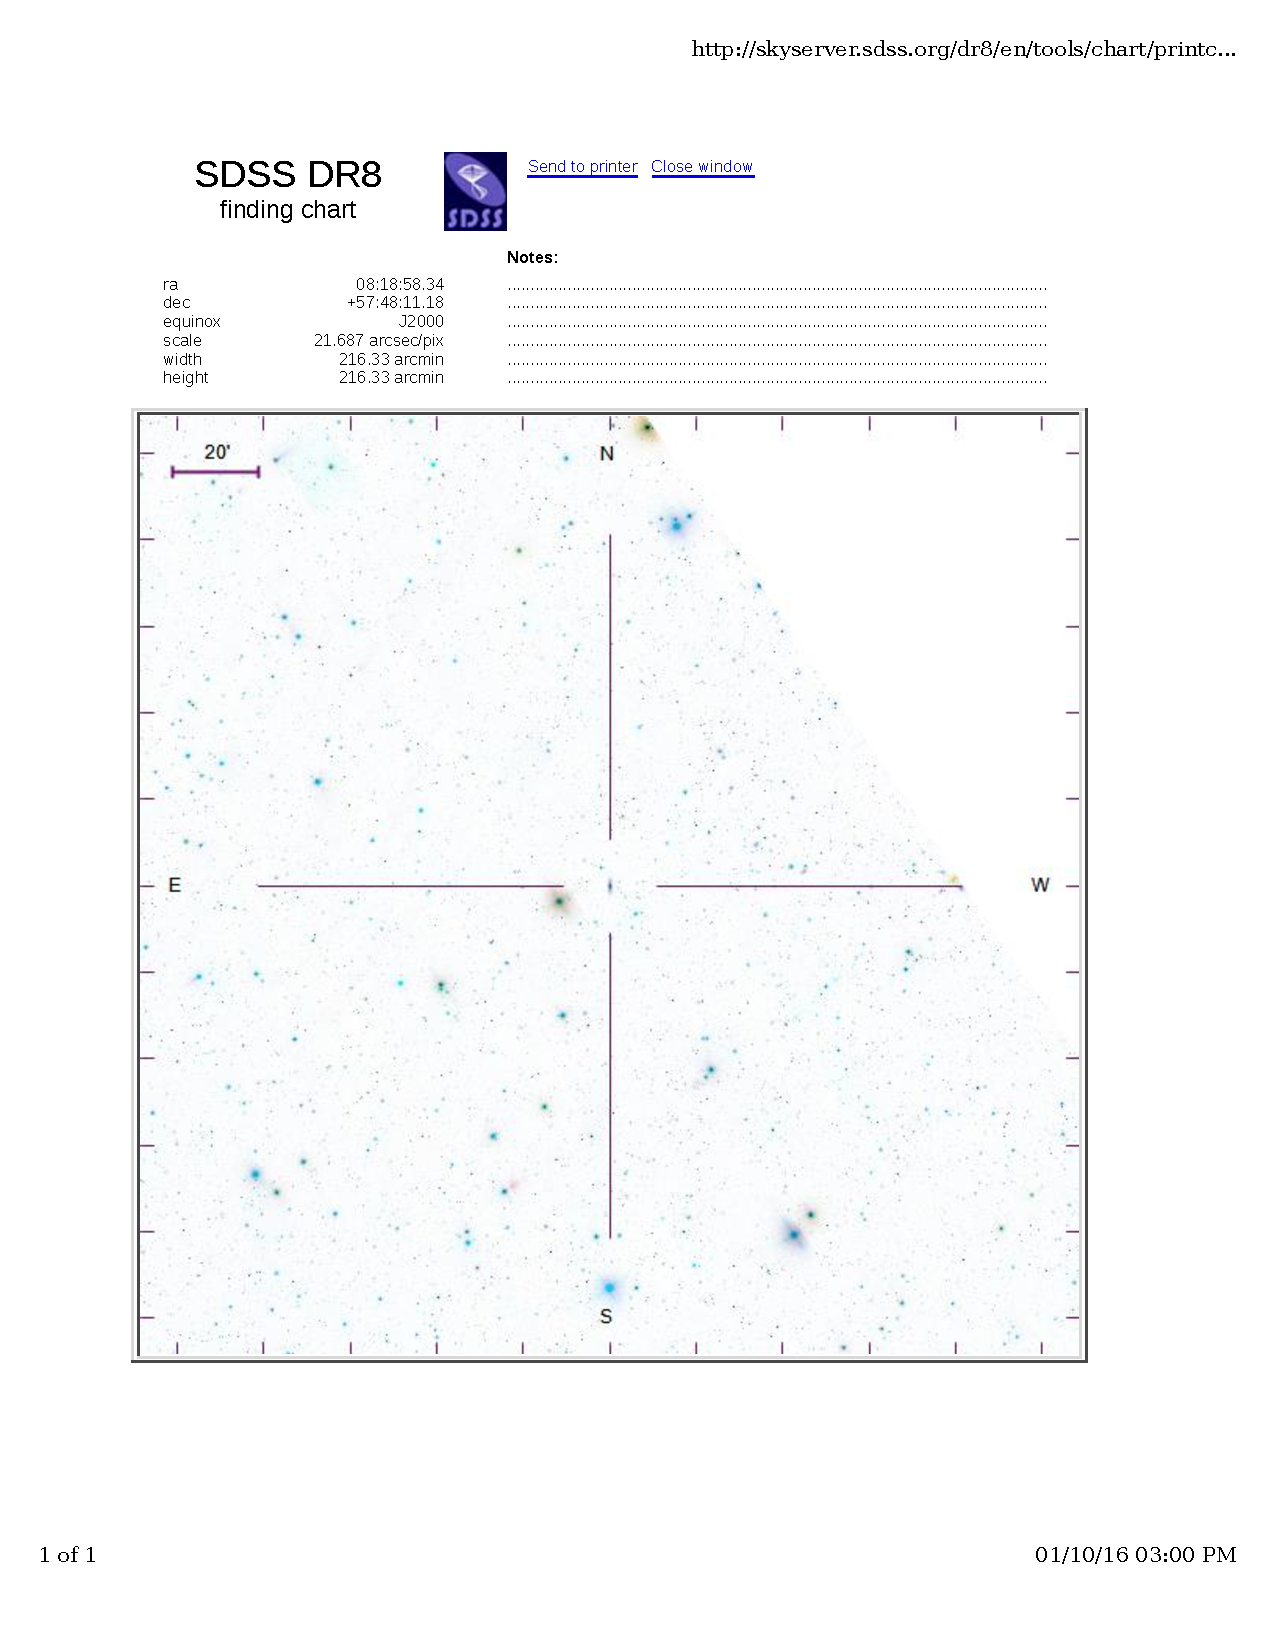
\includegraphics[scale=0.7]{figures/NGC2549.pdf}
\caption{NGC2549 SDSS DR8 Navigate Tool image with masks}
\end{figure}

\begin{figure}[h!]
\centering
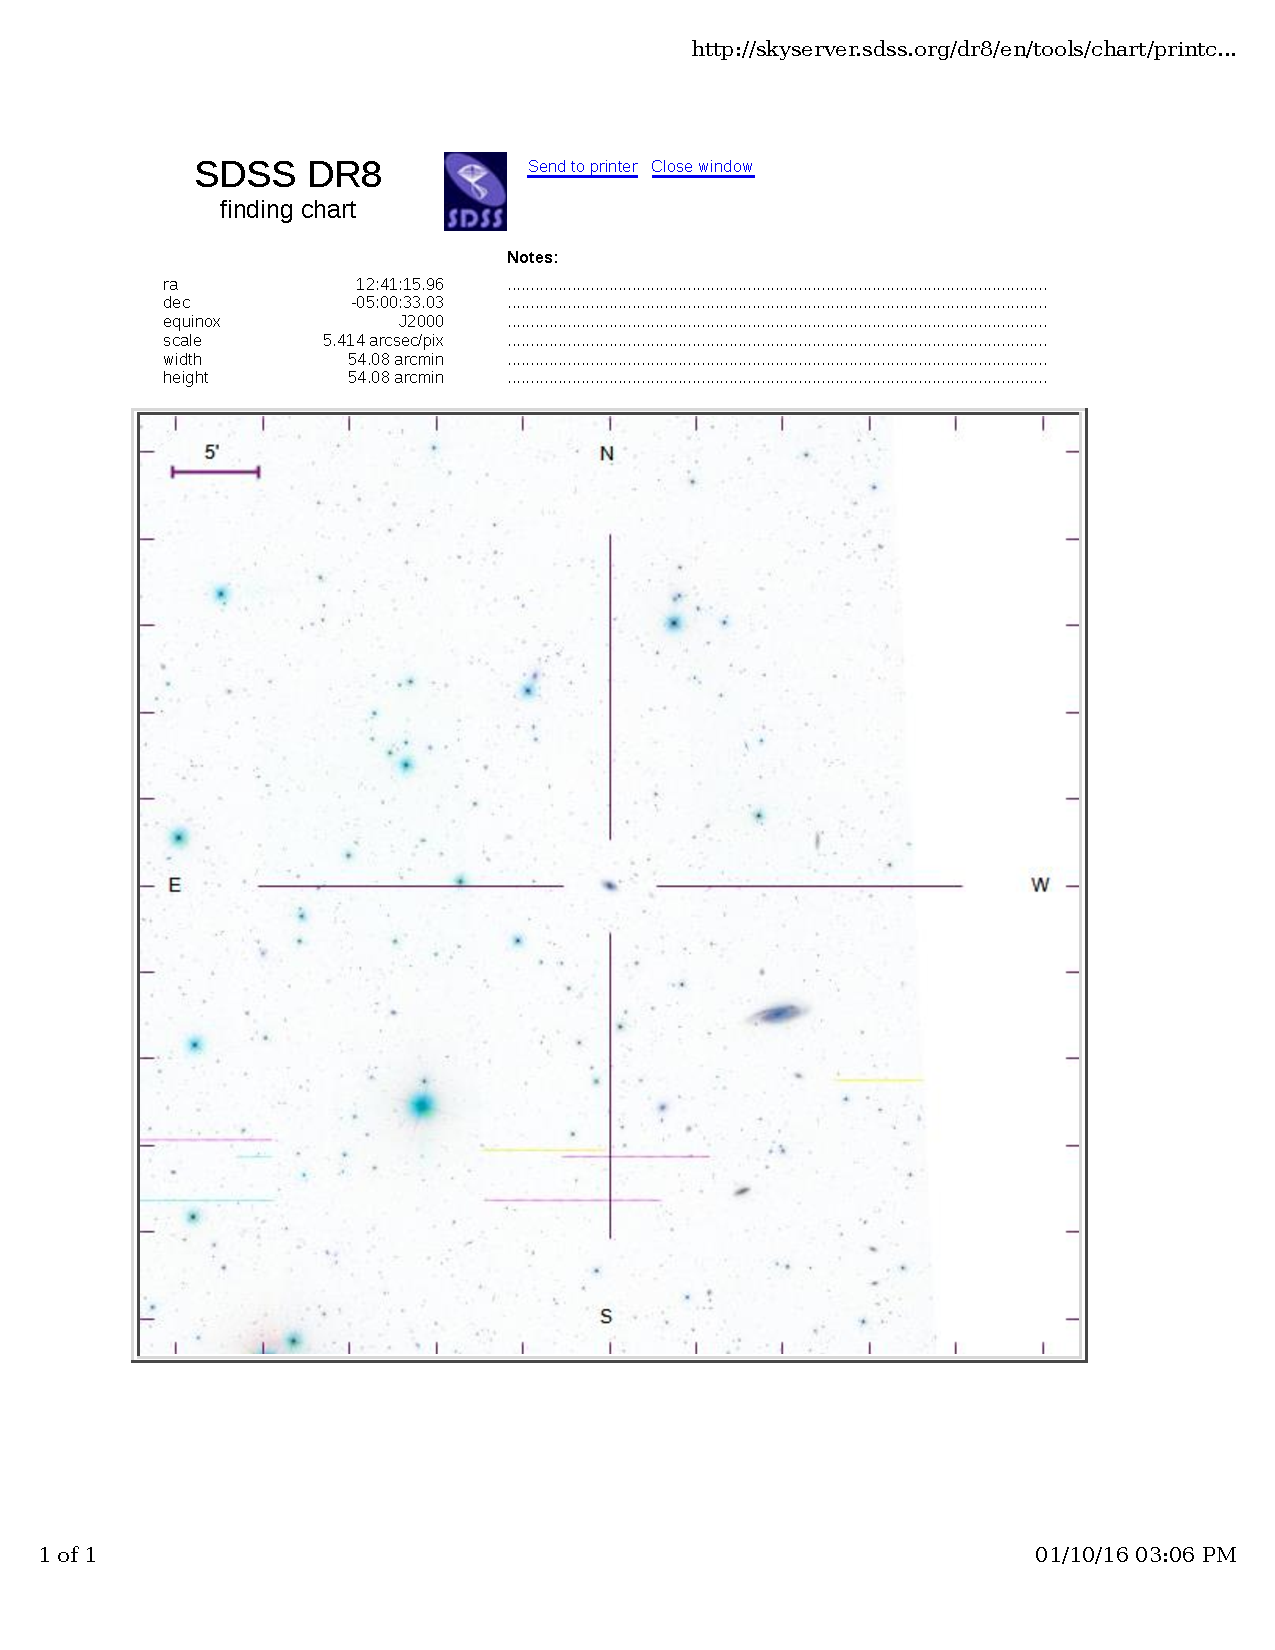
\includegraphics[scale=0.7]{figures/PGC042549.pdf}
\caption{PGC042549 SDSS DR8 Navigate Tool image with masks}
\end{figure}

\begin{figure}[h!]
\centering
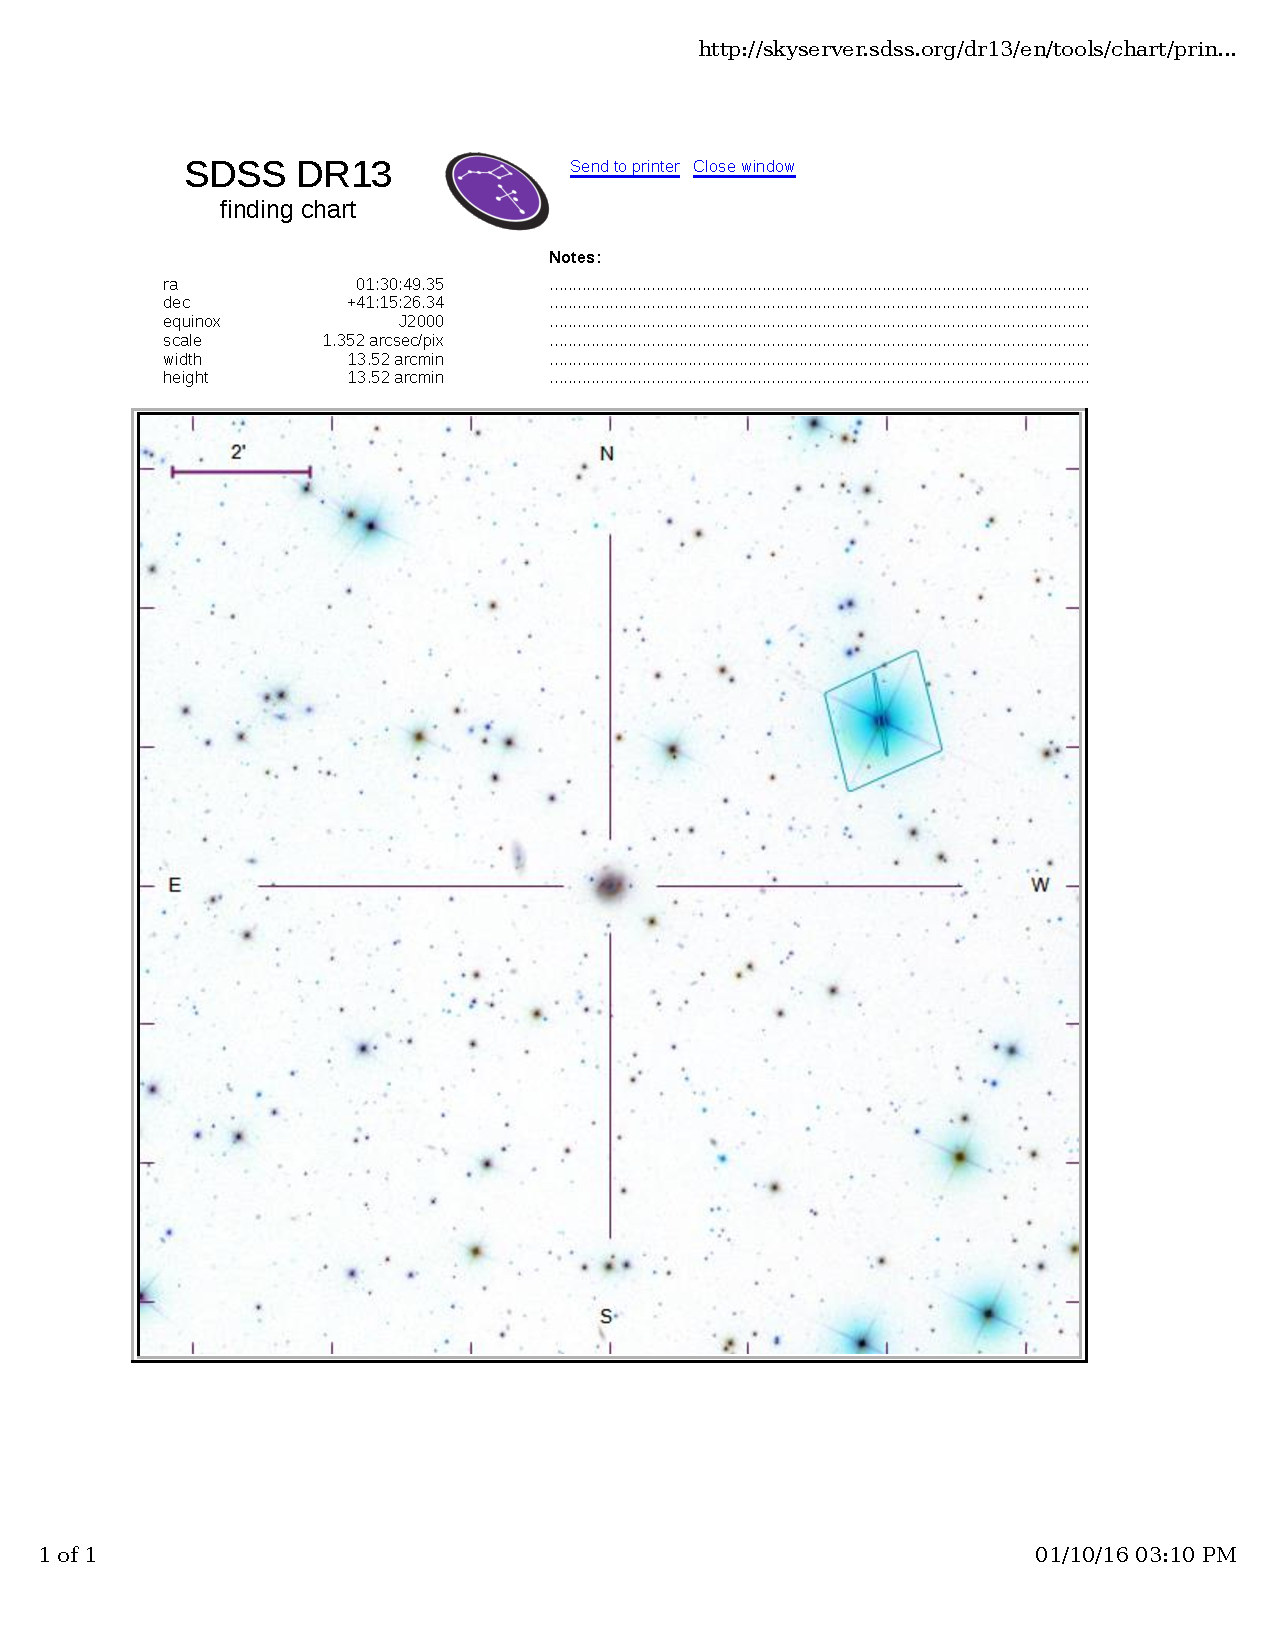
\includegraphics[scale=0.7]{figures/NGC0573.pdf}
\caption{NGC0573 SDSS DR8 Navigate Tool image with masks}
\end{figure}

\begin{figure}[h!]
\centering
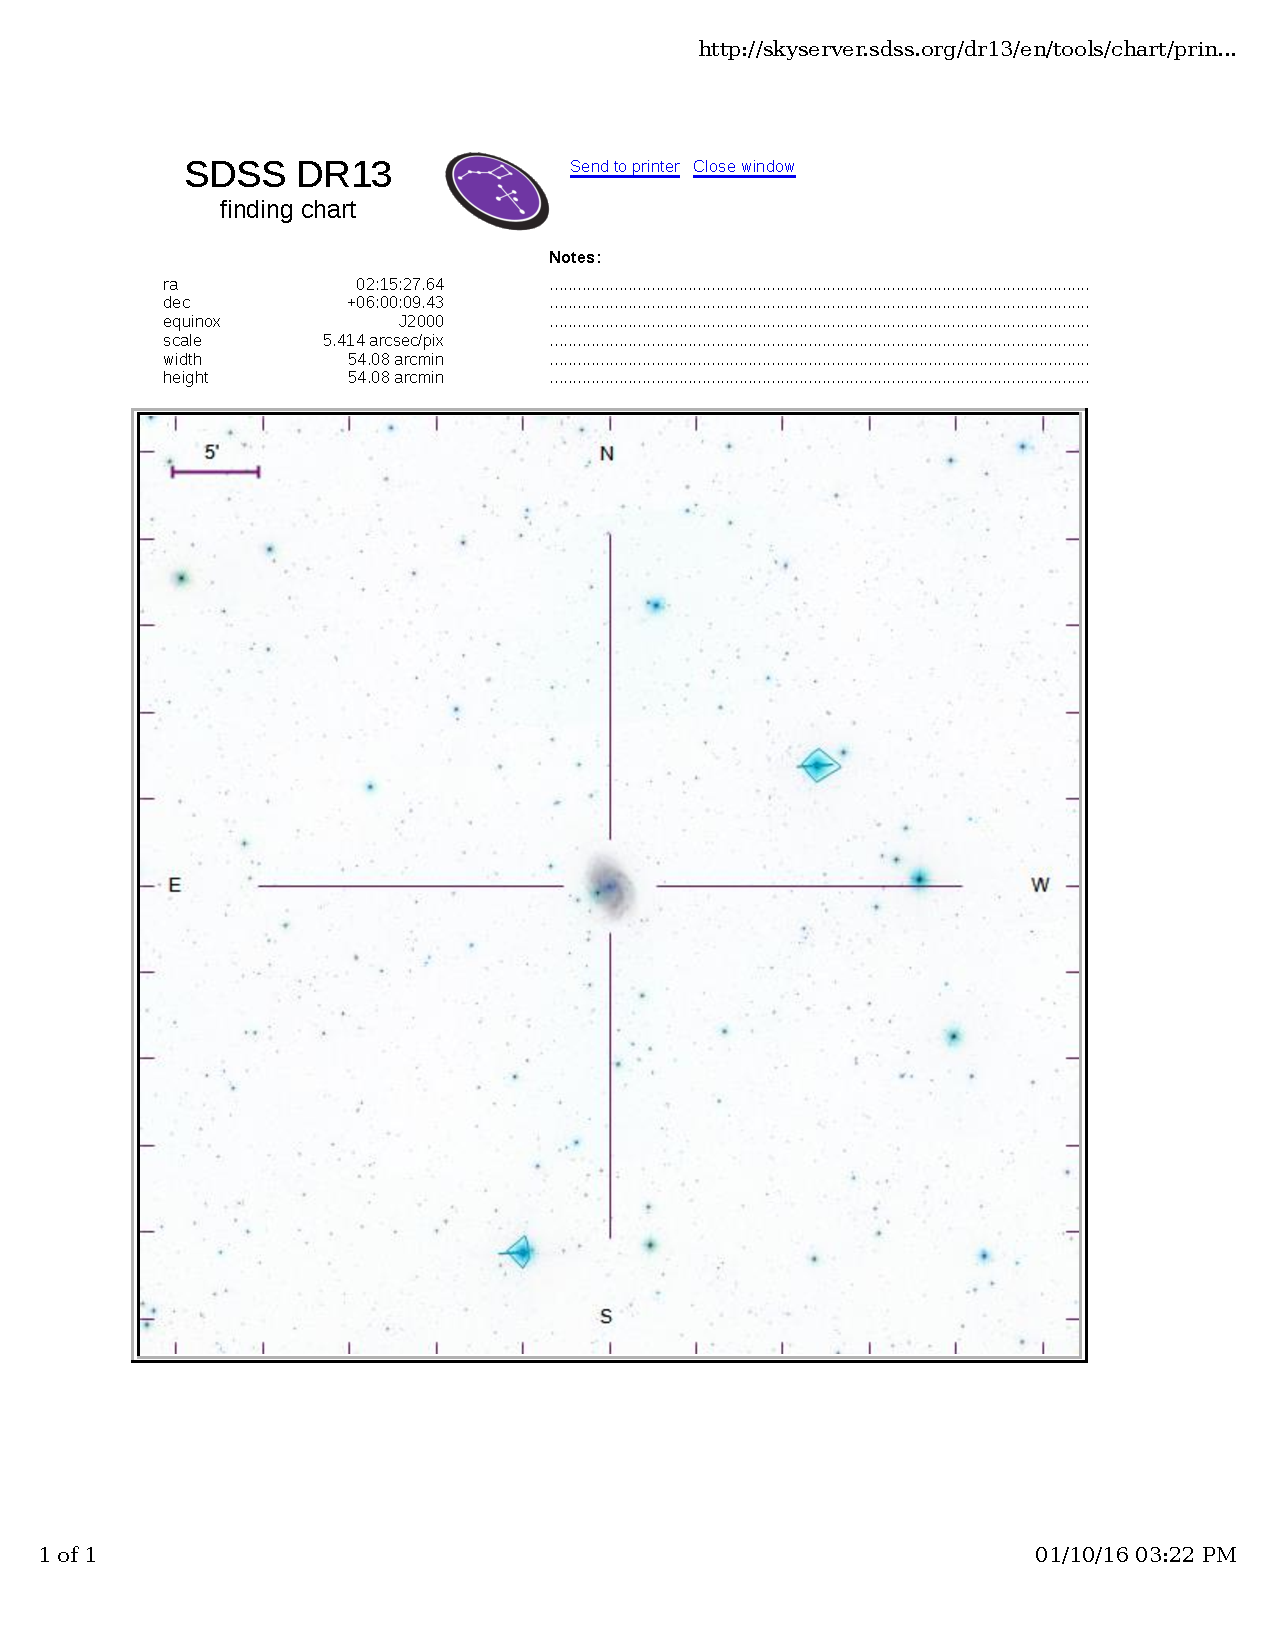
\includegraphics[scale=0.7]{figures/NGC0864.pdf}
\caption{NGC0864 SDSS DR8 Navigate Tool image with masks}
\end{figure}

\begin{figure}[h!]
\centering
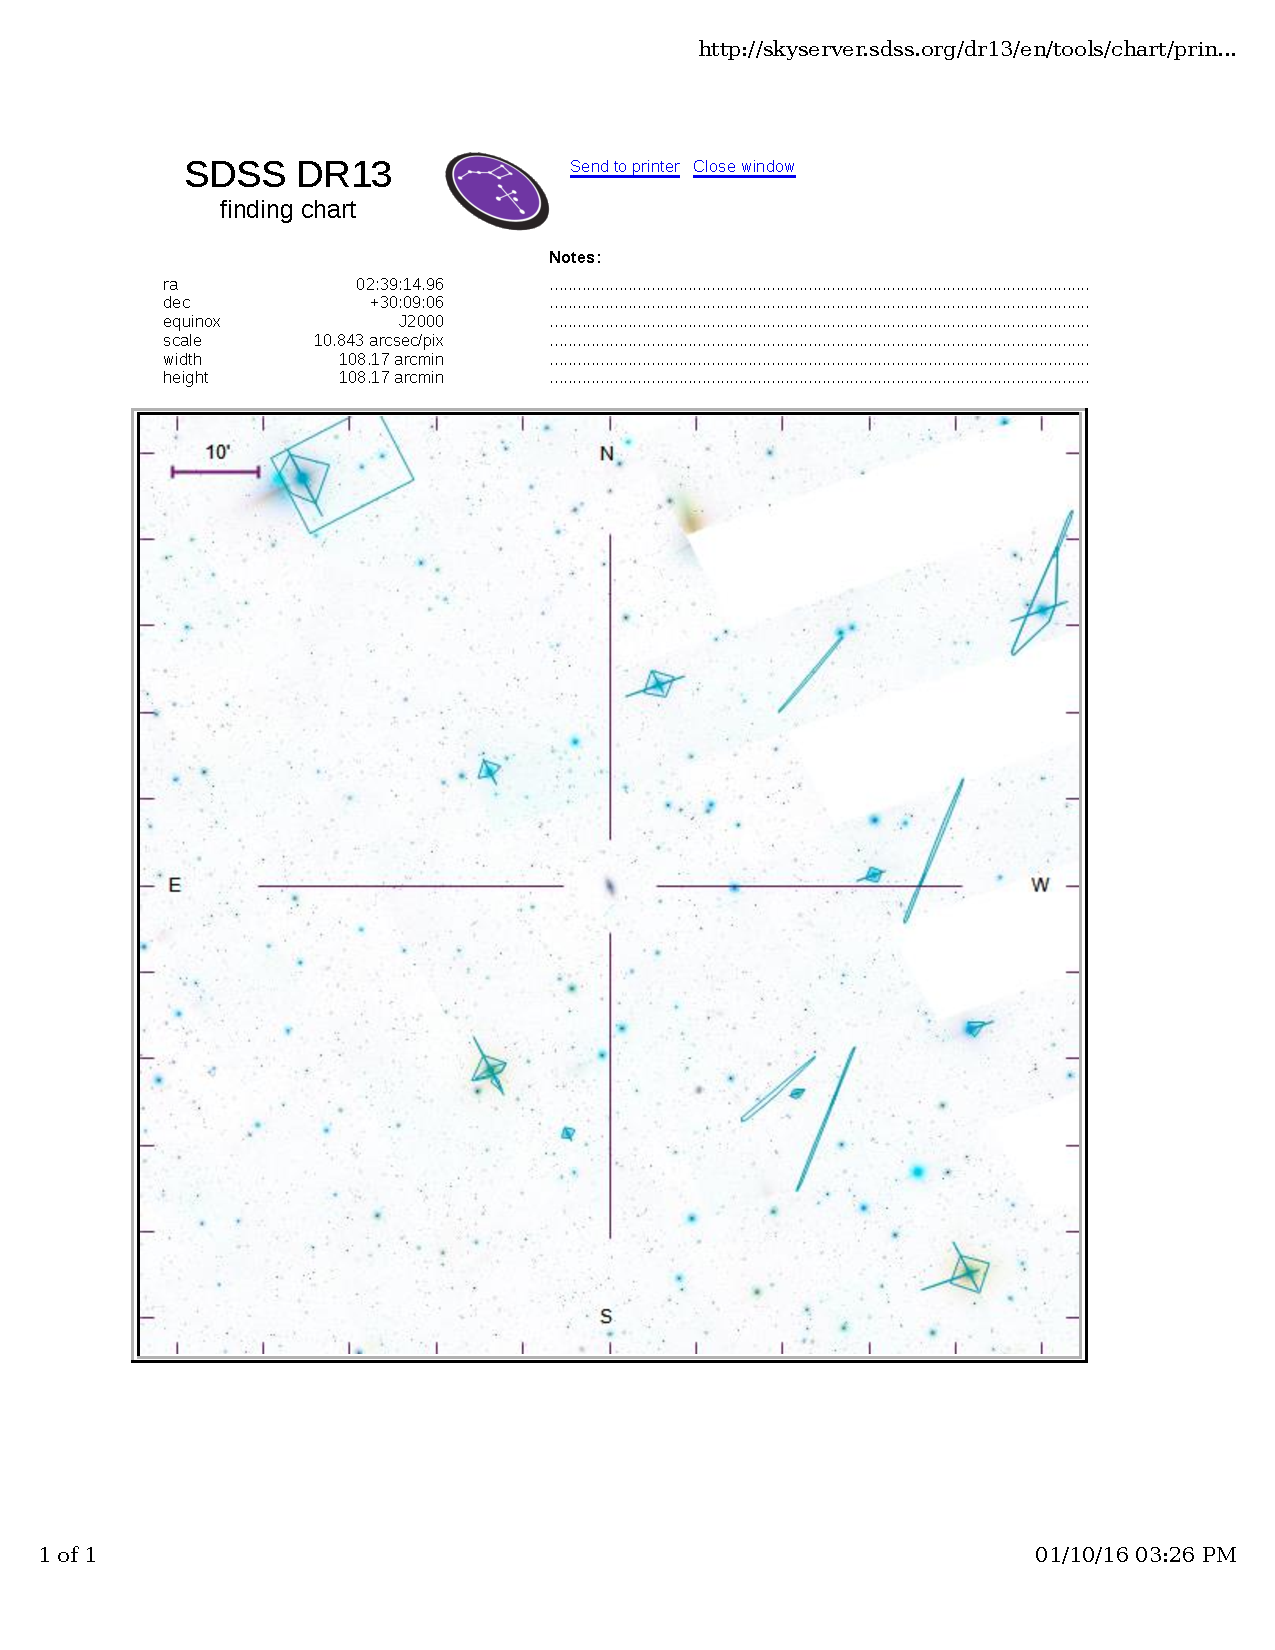
\includegraphics[scale=0.7]{figures/NGC1012.pdf}
\caption{NGC1012 SDSS DR8 Navigate Tool image with masks}
\end{figure}

\begin{figure}[h!]
\centering
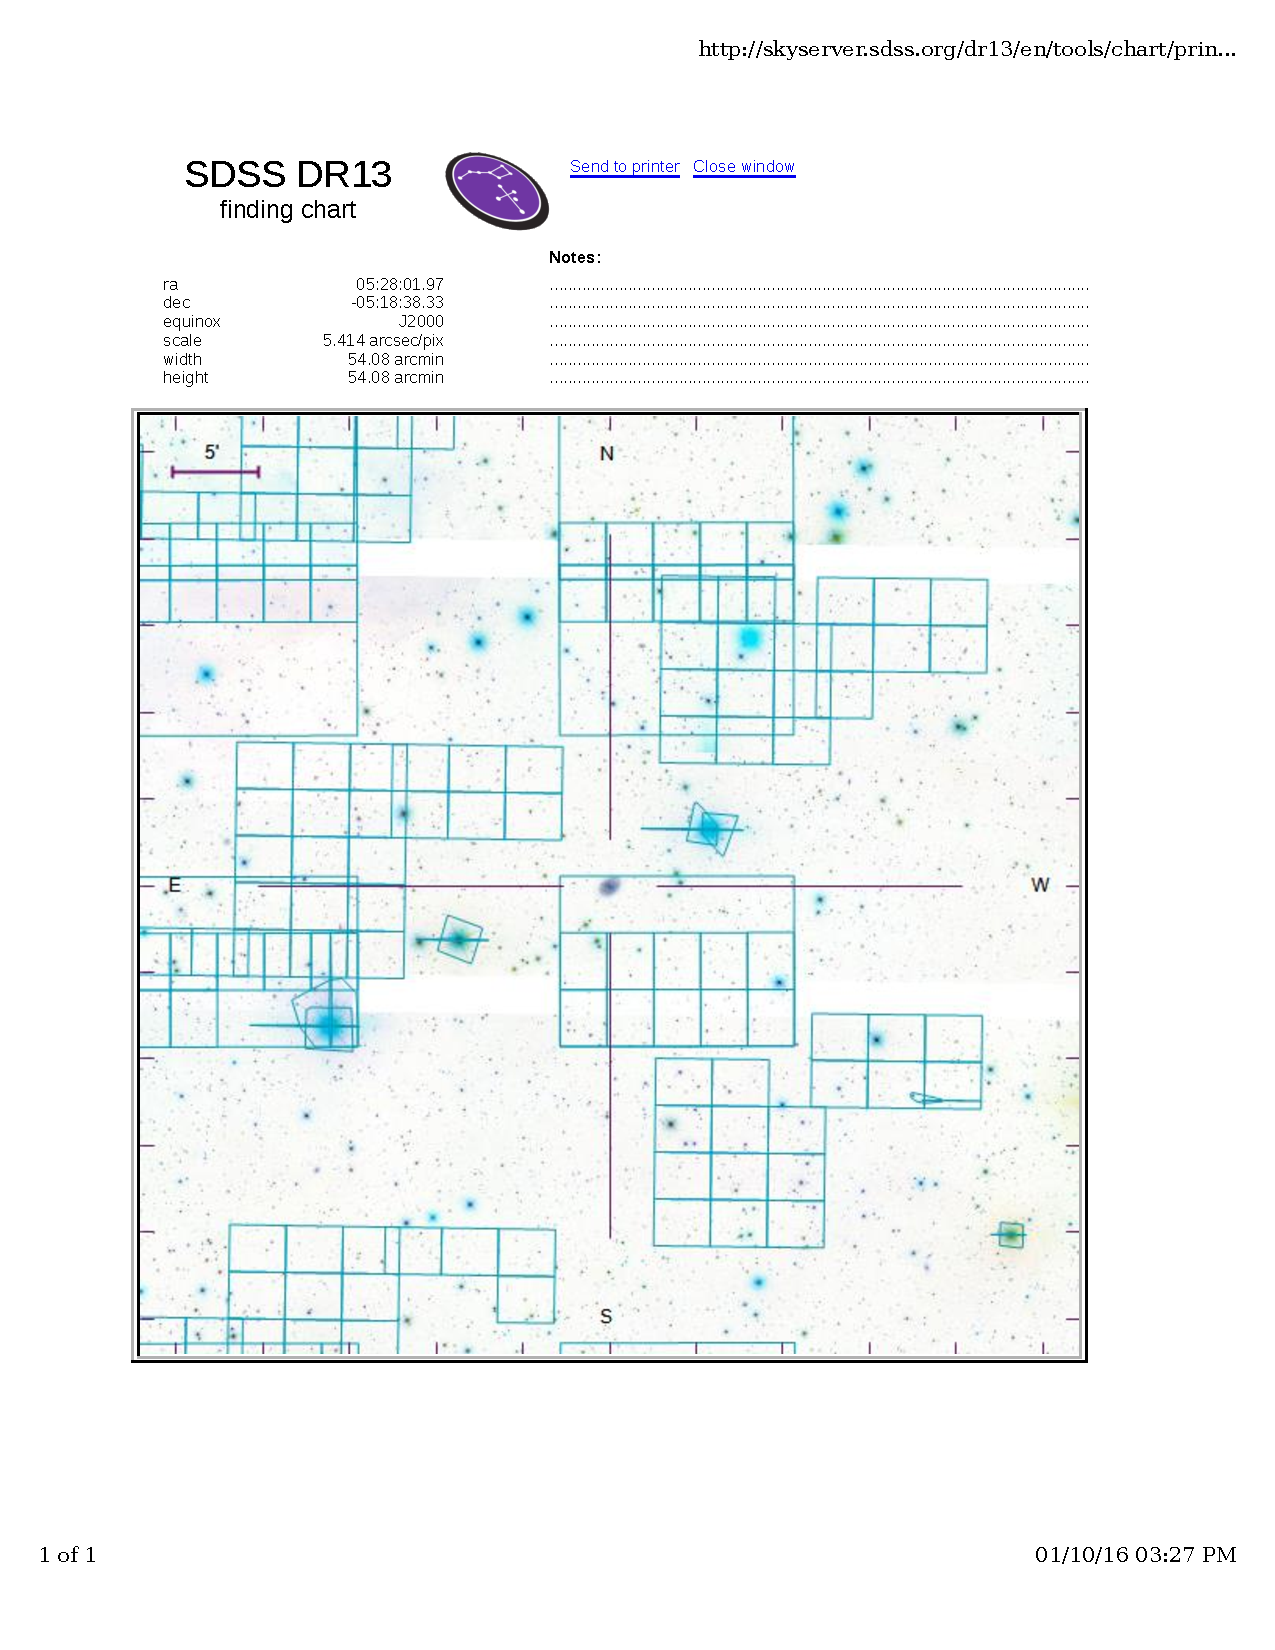
\includegraphics[scale=0.7]{figures/NGC1924.pdf}
\caption{NGC1924 SDSS DR8 Navigate Tool image with masks}
\end{figure}

\begin{figure}[h!]
\centering
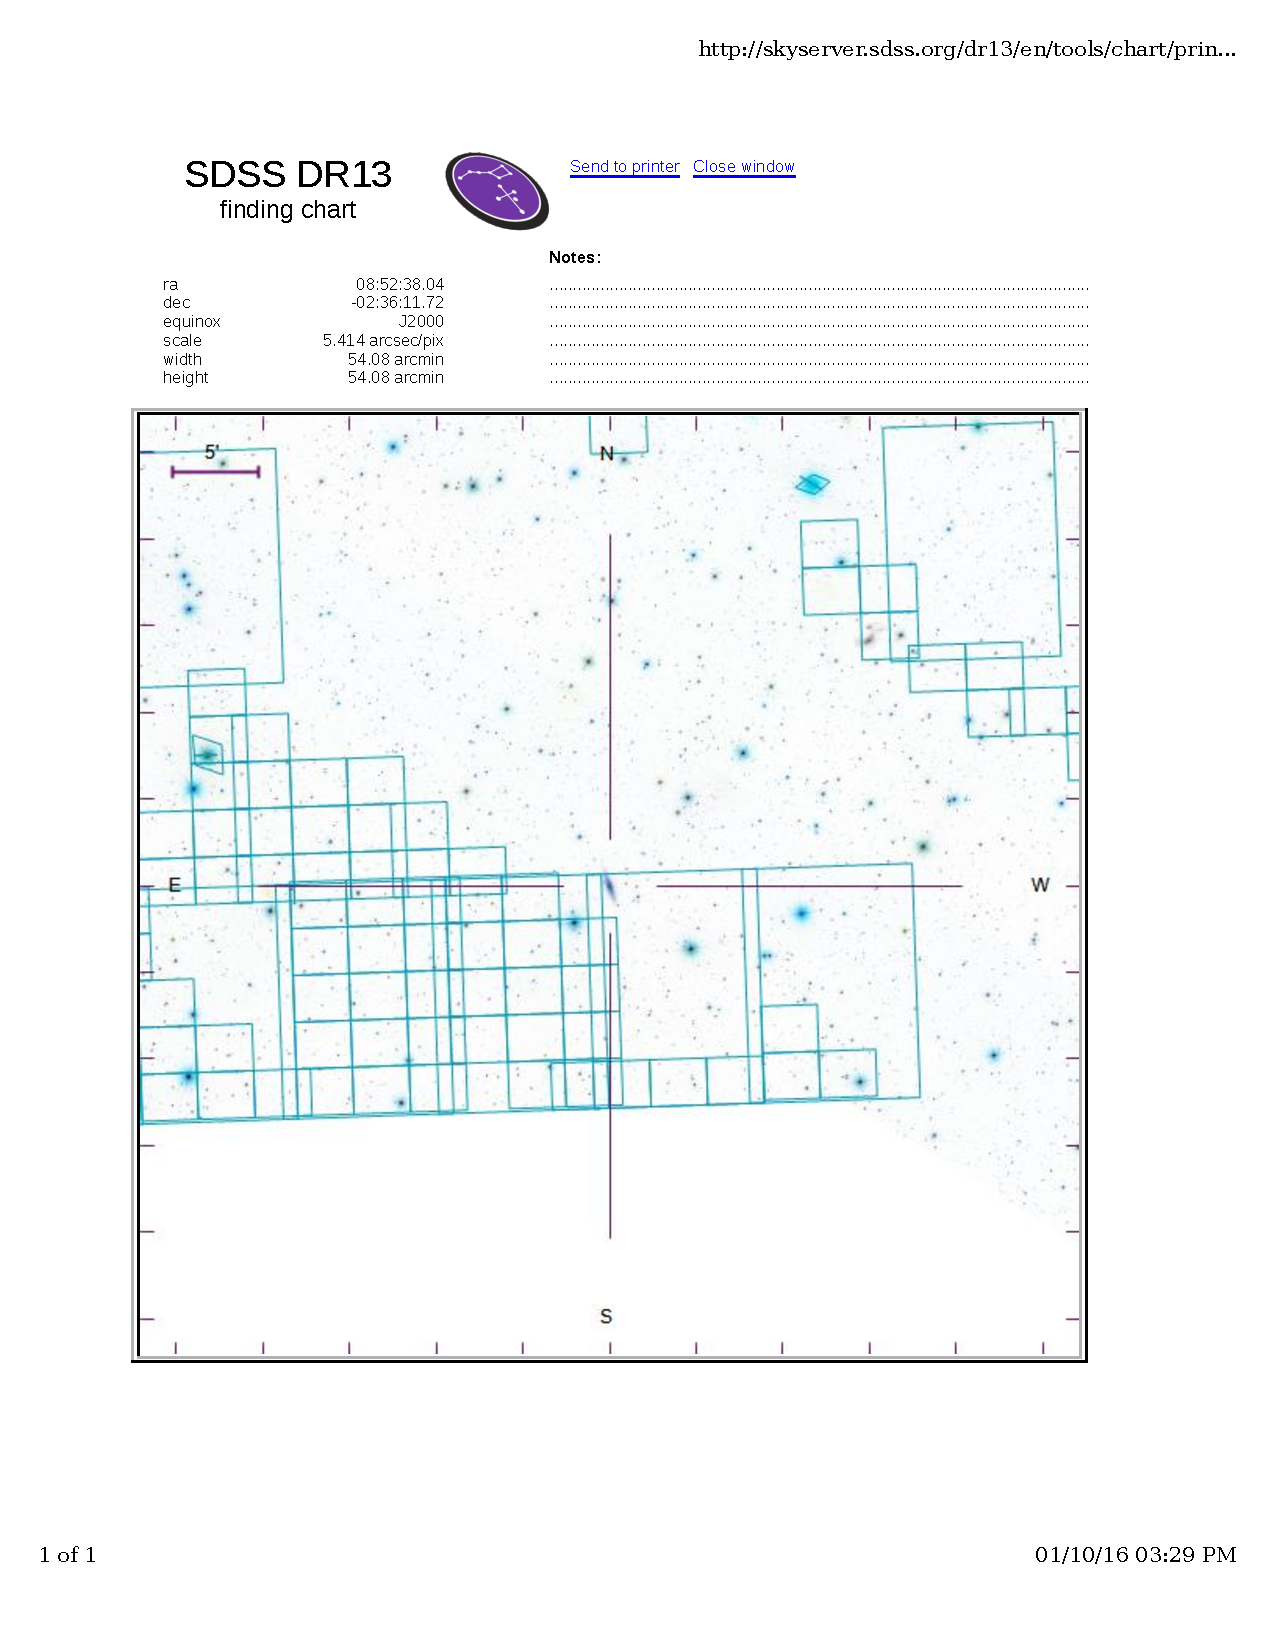
\includegraphics[scale=0.7]{figures/NGC2690.pdf}
\caption{NGC2690 SDSS DR8 Navigate Tool image with masks}
\end{figure}

\begin{figure}[h!]
\centering
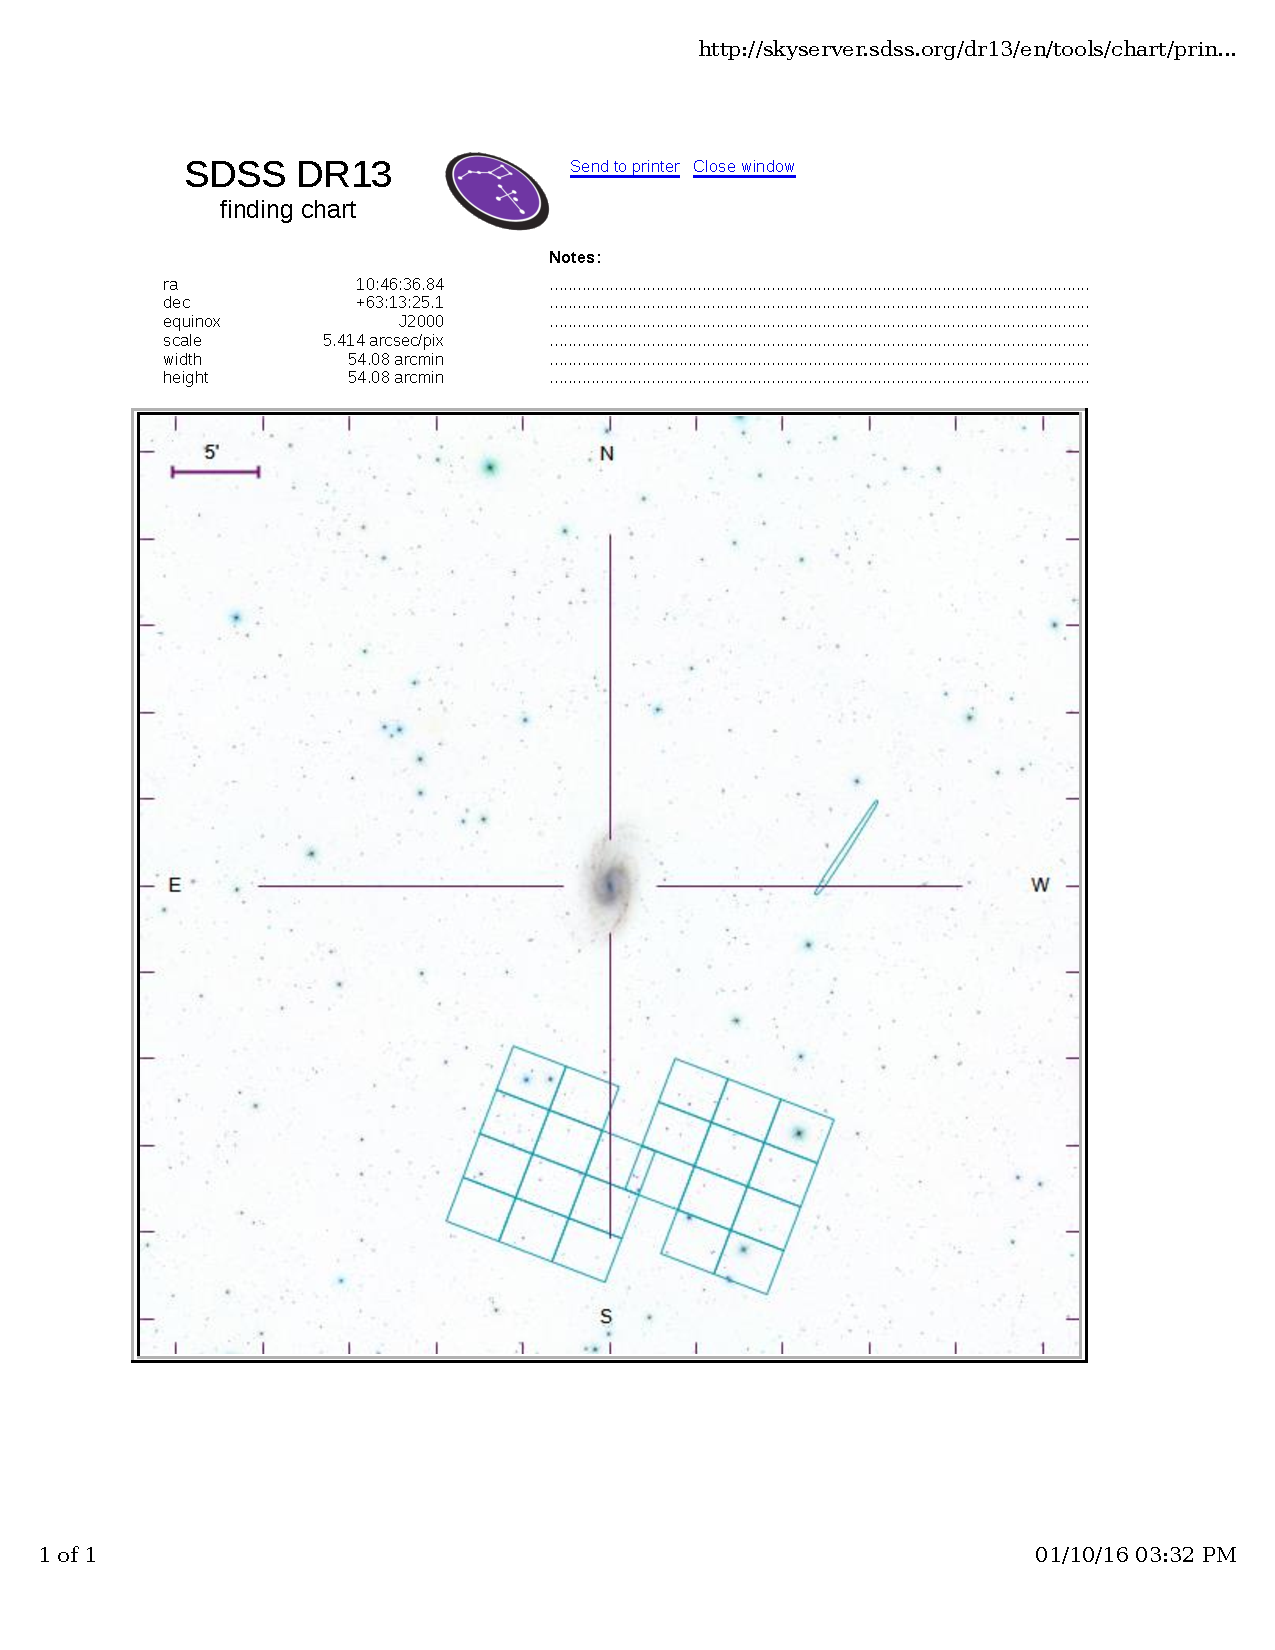
\includegraphics[scale=0.7]{figures/NGC3359.pdf}
\caption{NGC3359 SDSS DR8 Navigate Tool image with masks}
\end{figure}

\begin{figure}[h!]
\centering
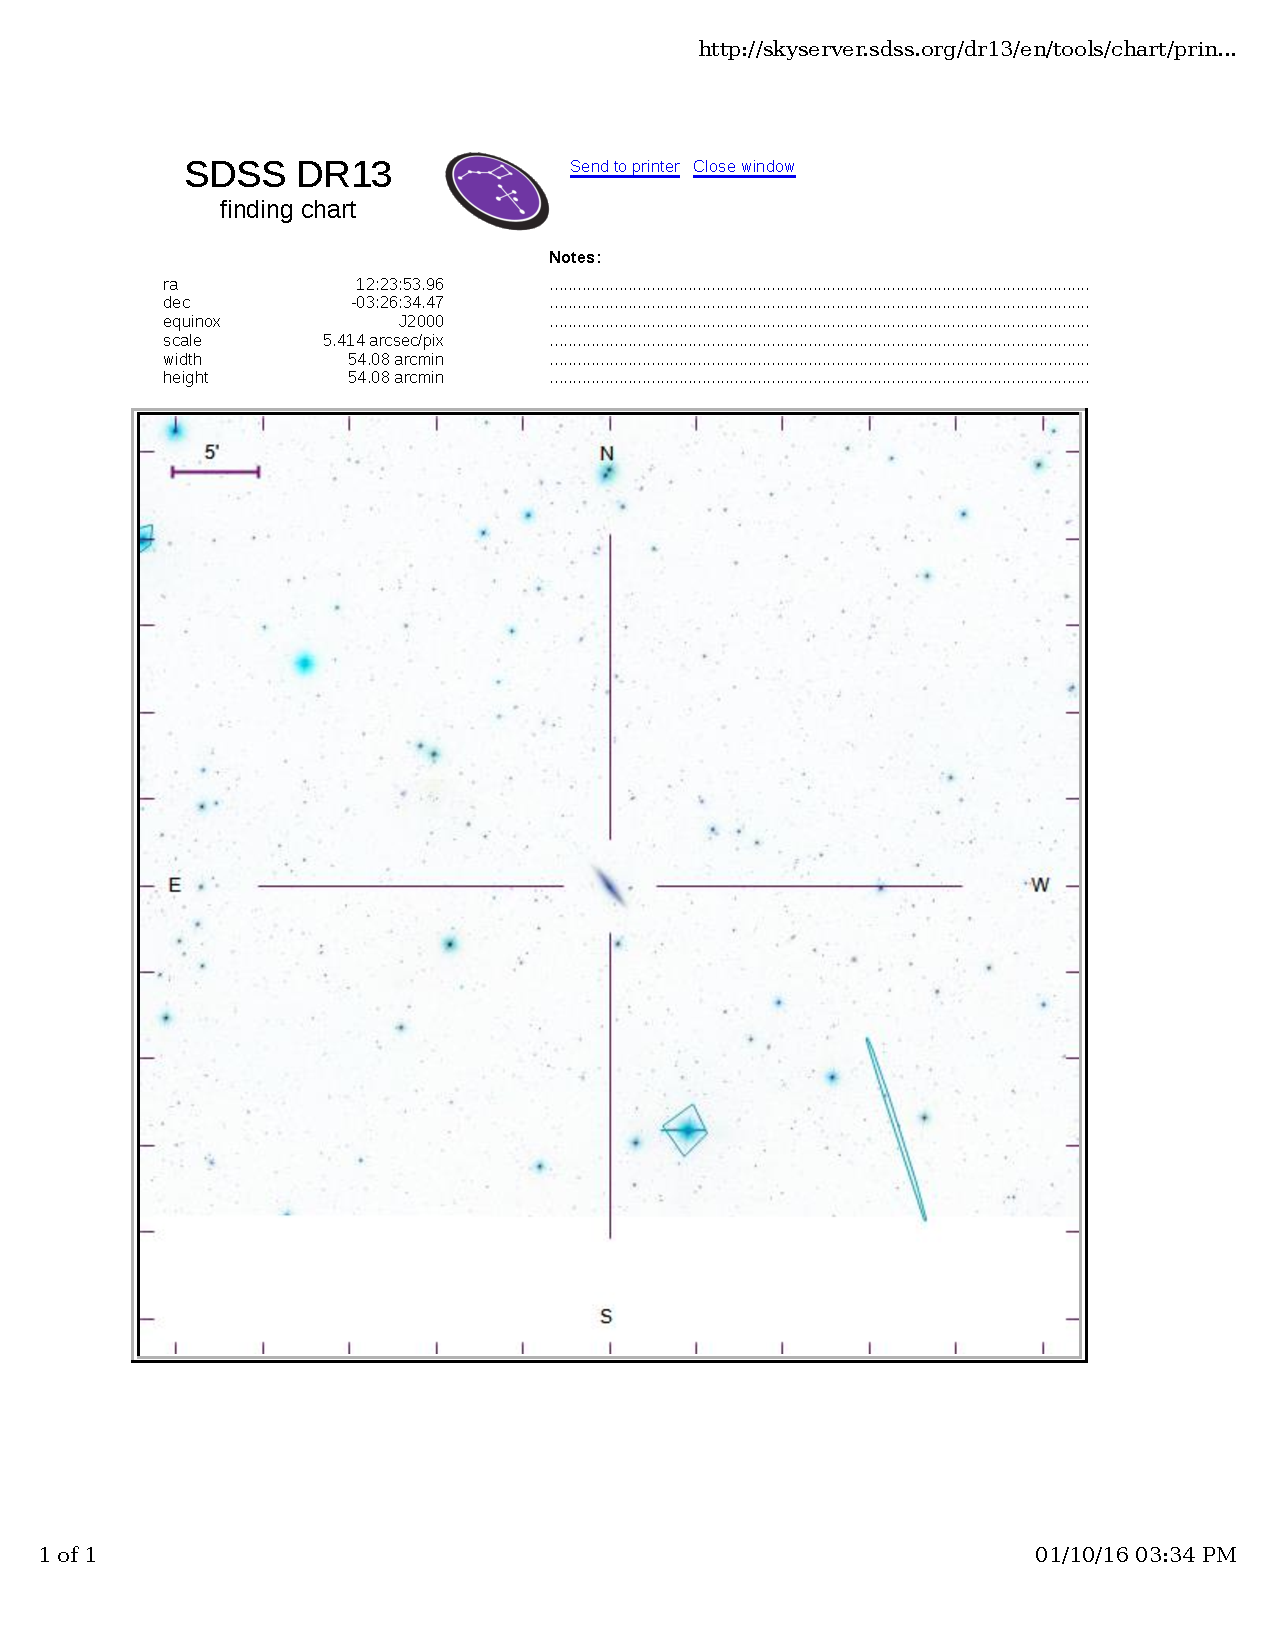
\includegraphics[scale=0.7]{figures/NGC4348.pdf}
\caption{NGC4348 SDSS DR8 Navigate Tool image with masks}
\end{figure}

\begin{figure}[h!]
\centering
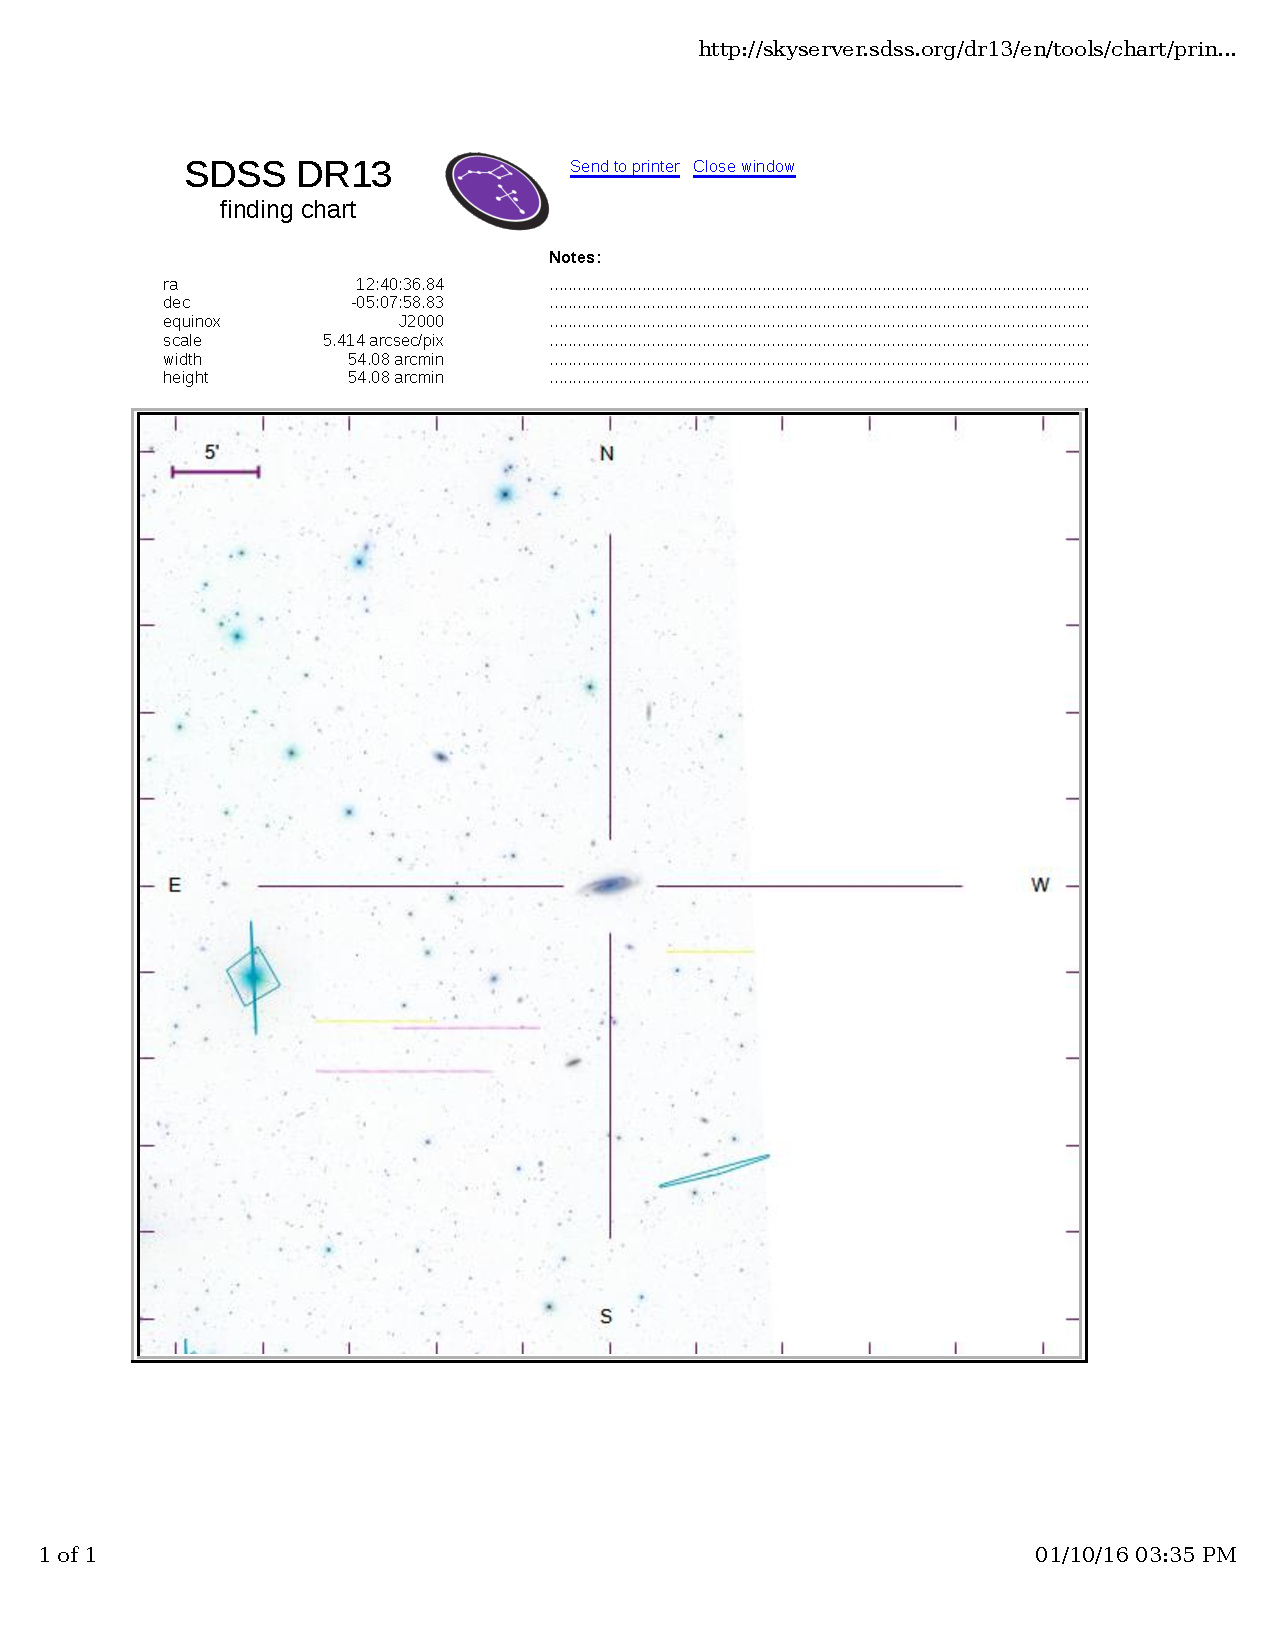
\includegraphics[scale=0.7]{figures/NGC4602.pdf}
\caption{NGC4602 SDSS DR8 Navigate Tool image with masks}
\end{figure}

\begin{figure}[h!]
\centering
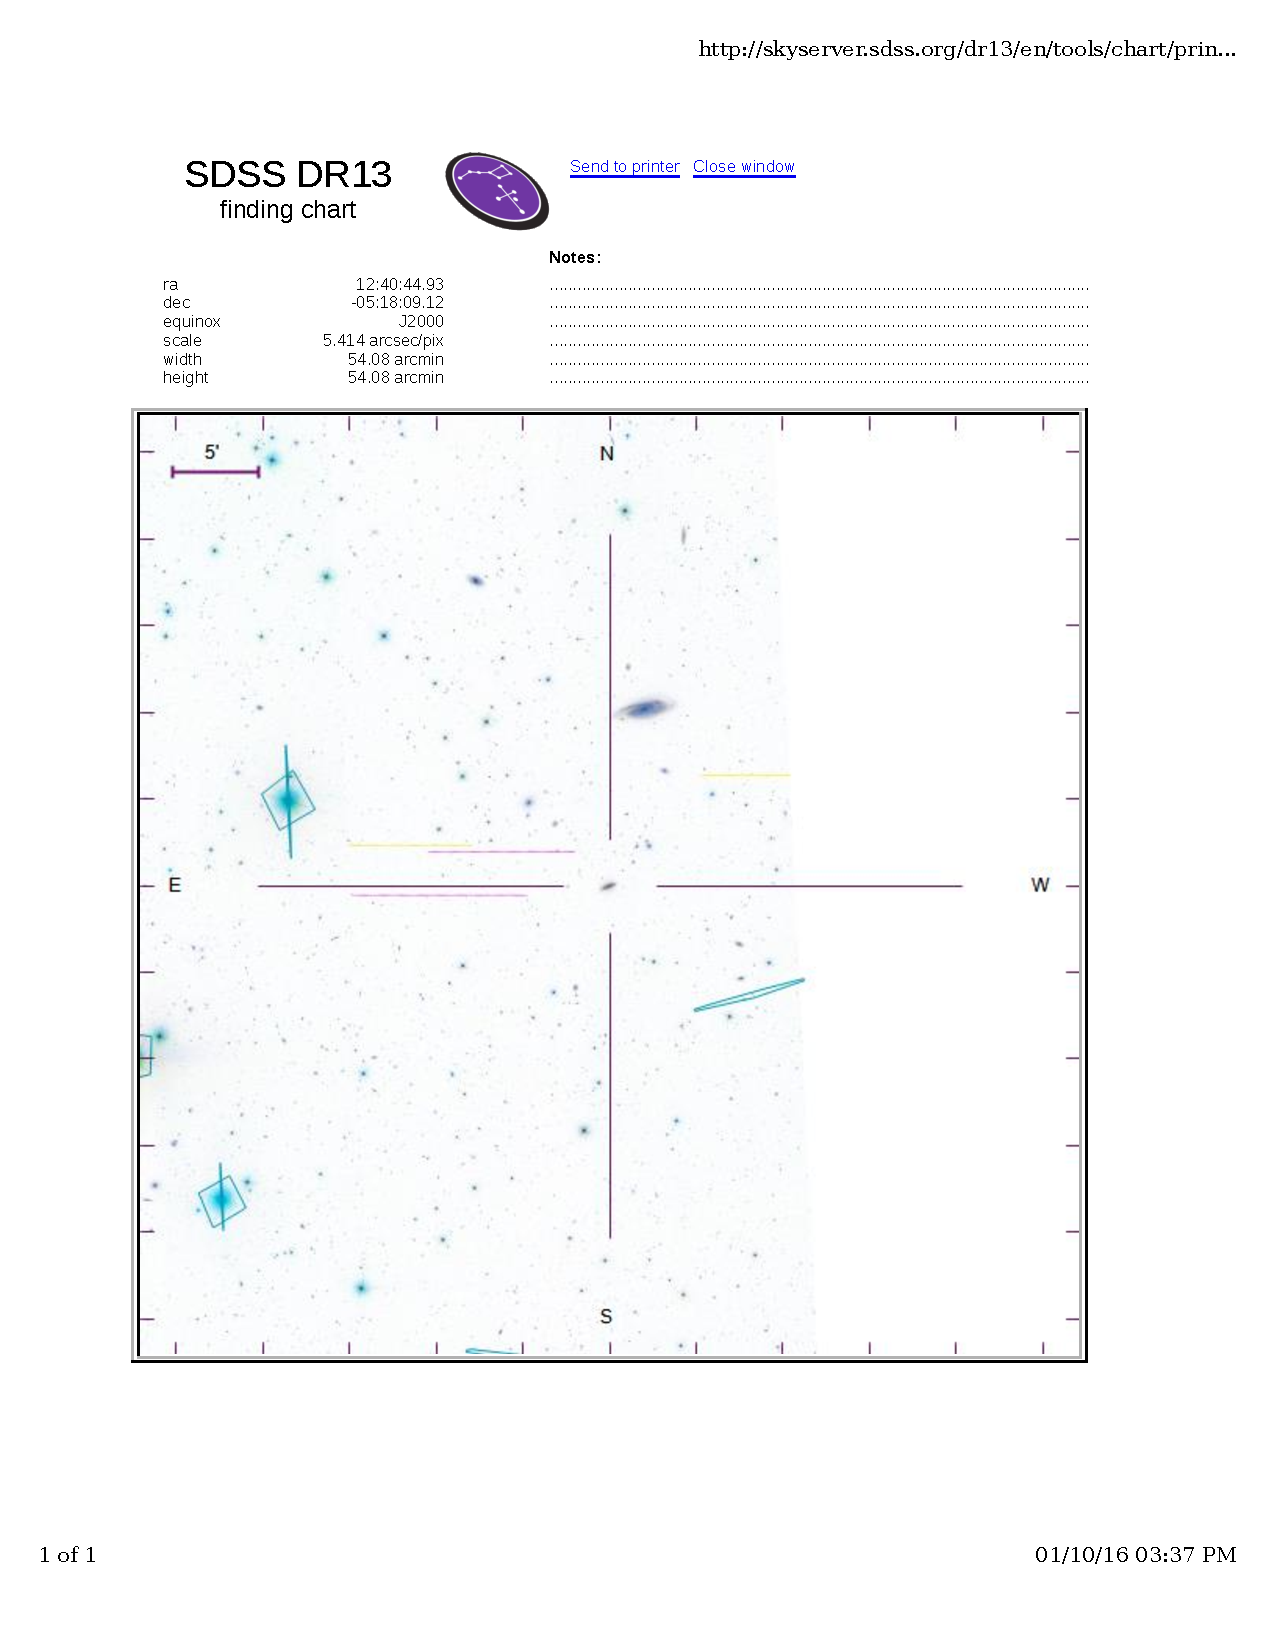
\includegraphics[scale=0.7]{figures/NGC4604.pdf}
\caption{NGC4604 SDSS DR8 Navigate Tool image with masks}
\end{figure}

\begin{figure}[h!]
\centering
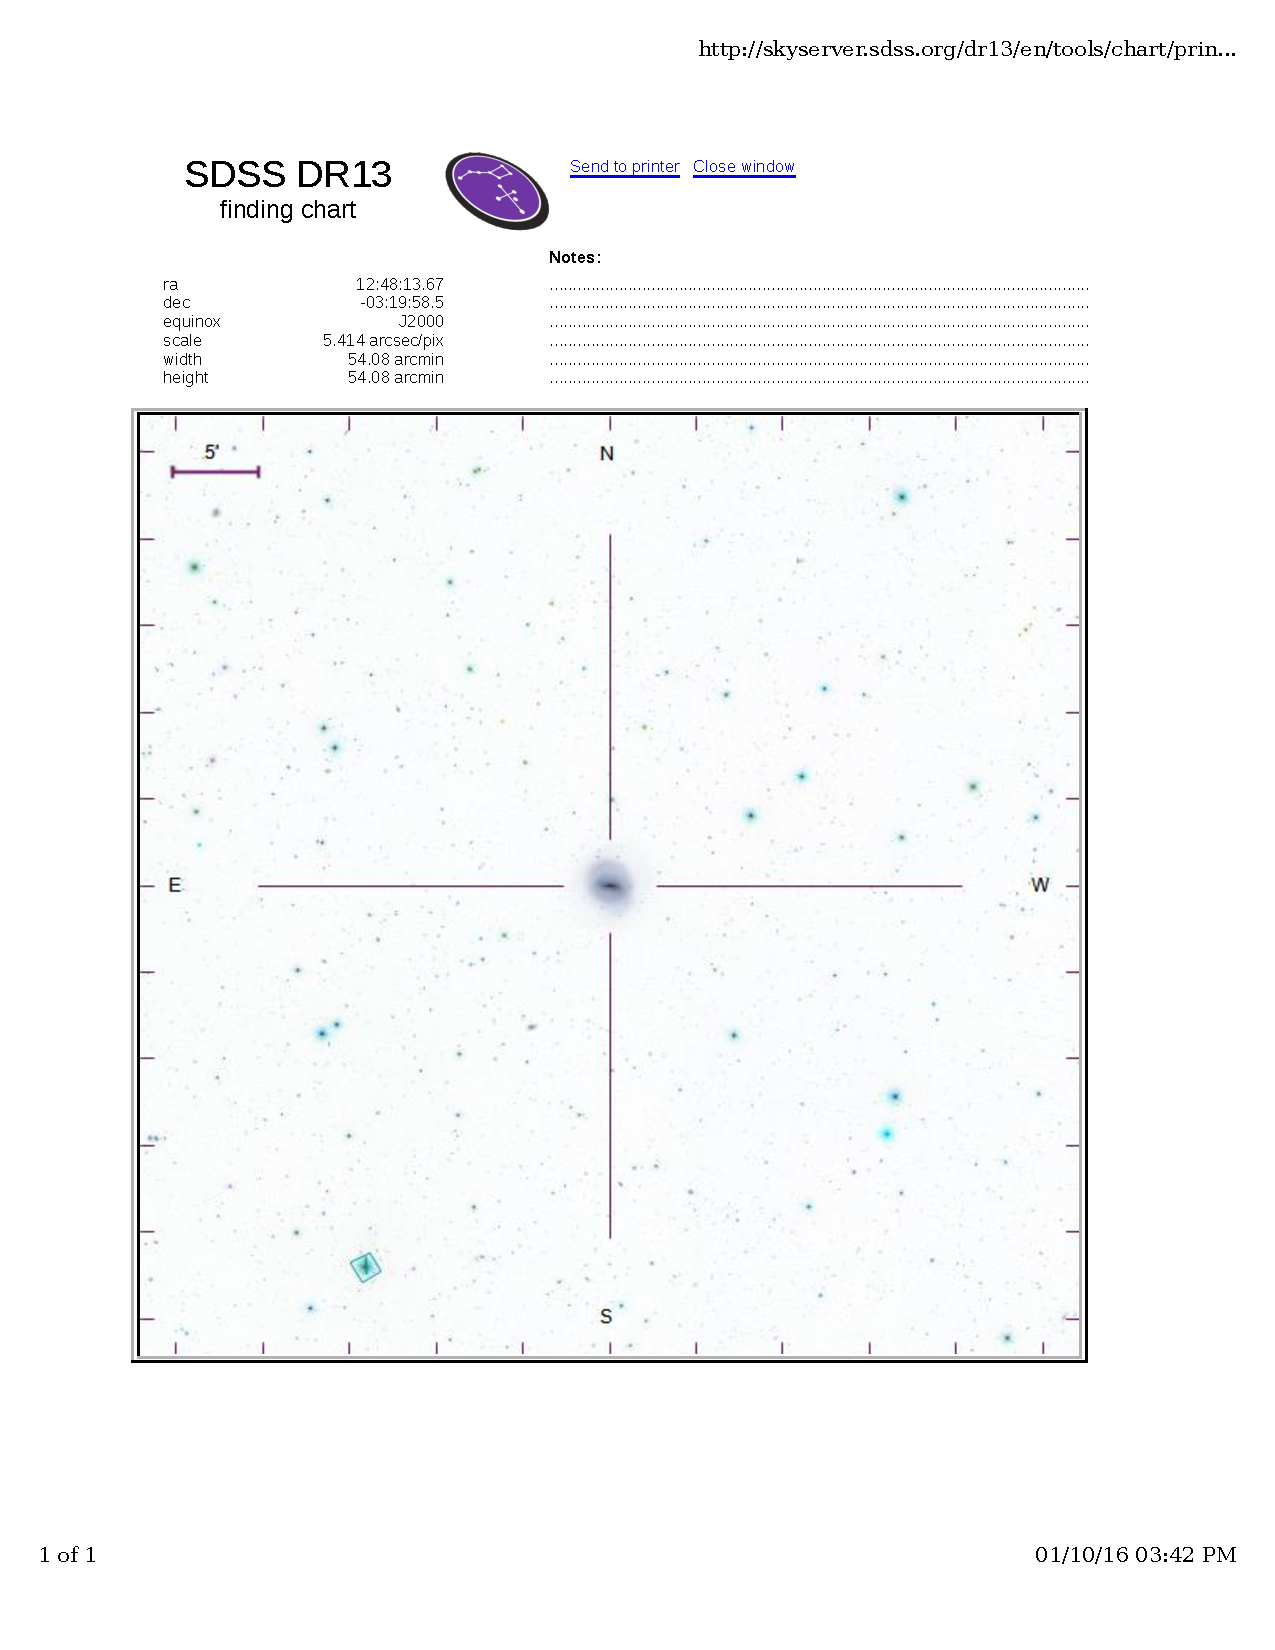
\includegraphics[scale=0.7]{figures/NGC4691.pdf}
\caption{NGC4691 SDSS DR8 Navigate Tool image with masks}
\end{figure}

\begin{figure}[h!]
\centering
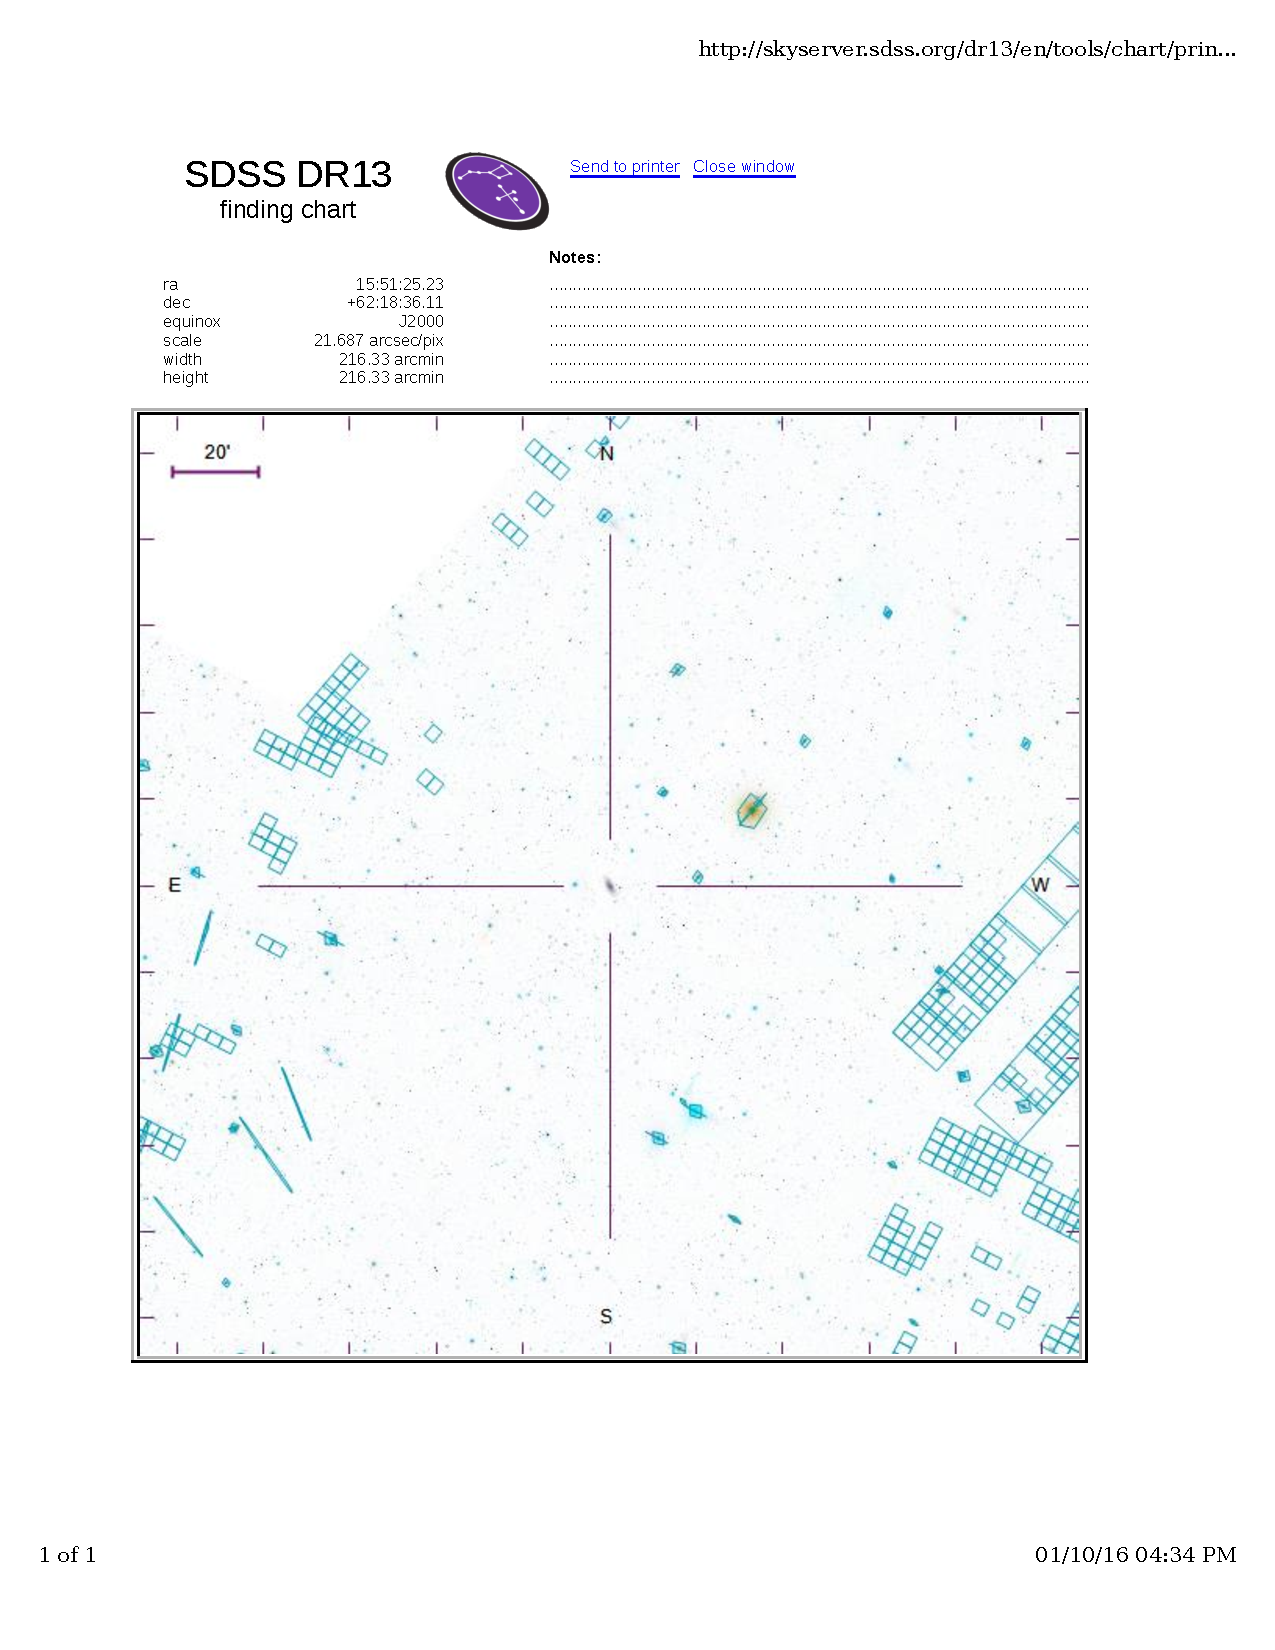
\includegraphics[scale=0.7]{figures/NGC6015.pdf}
\caption{NGC6015 SDSS DR8 Navigate Tool image with masks}
\end{figure}

\begin{figure}[h!]
\centering
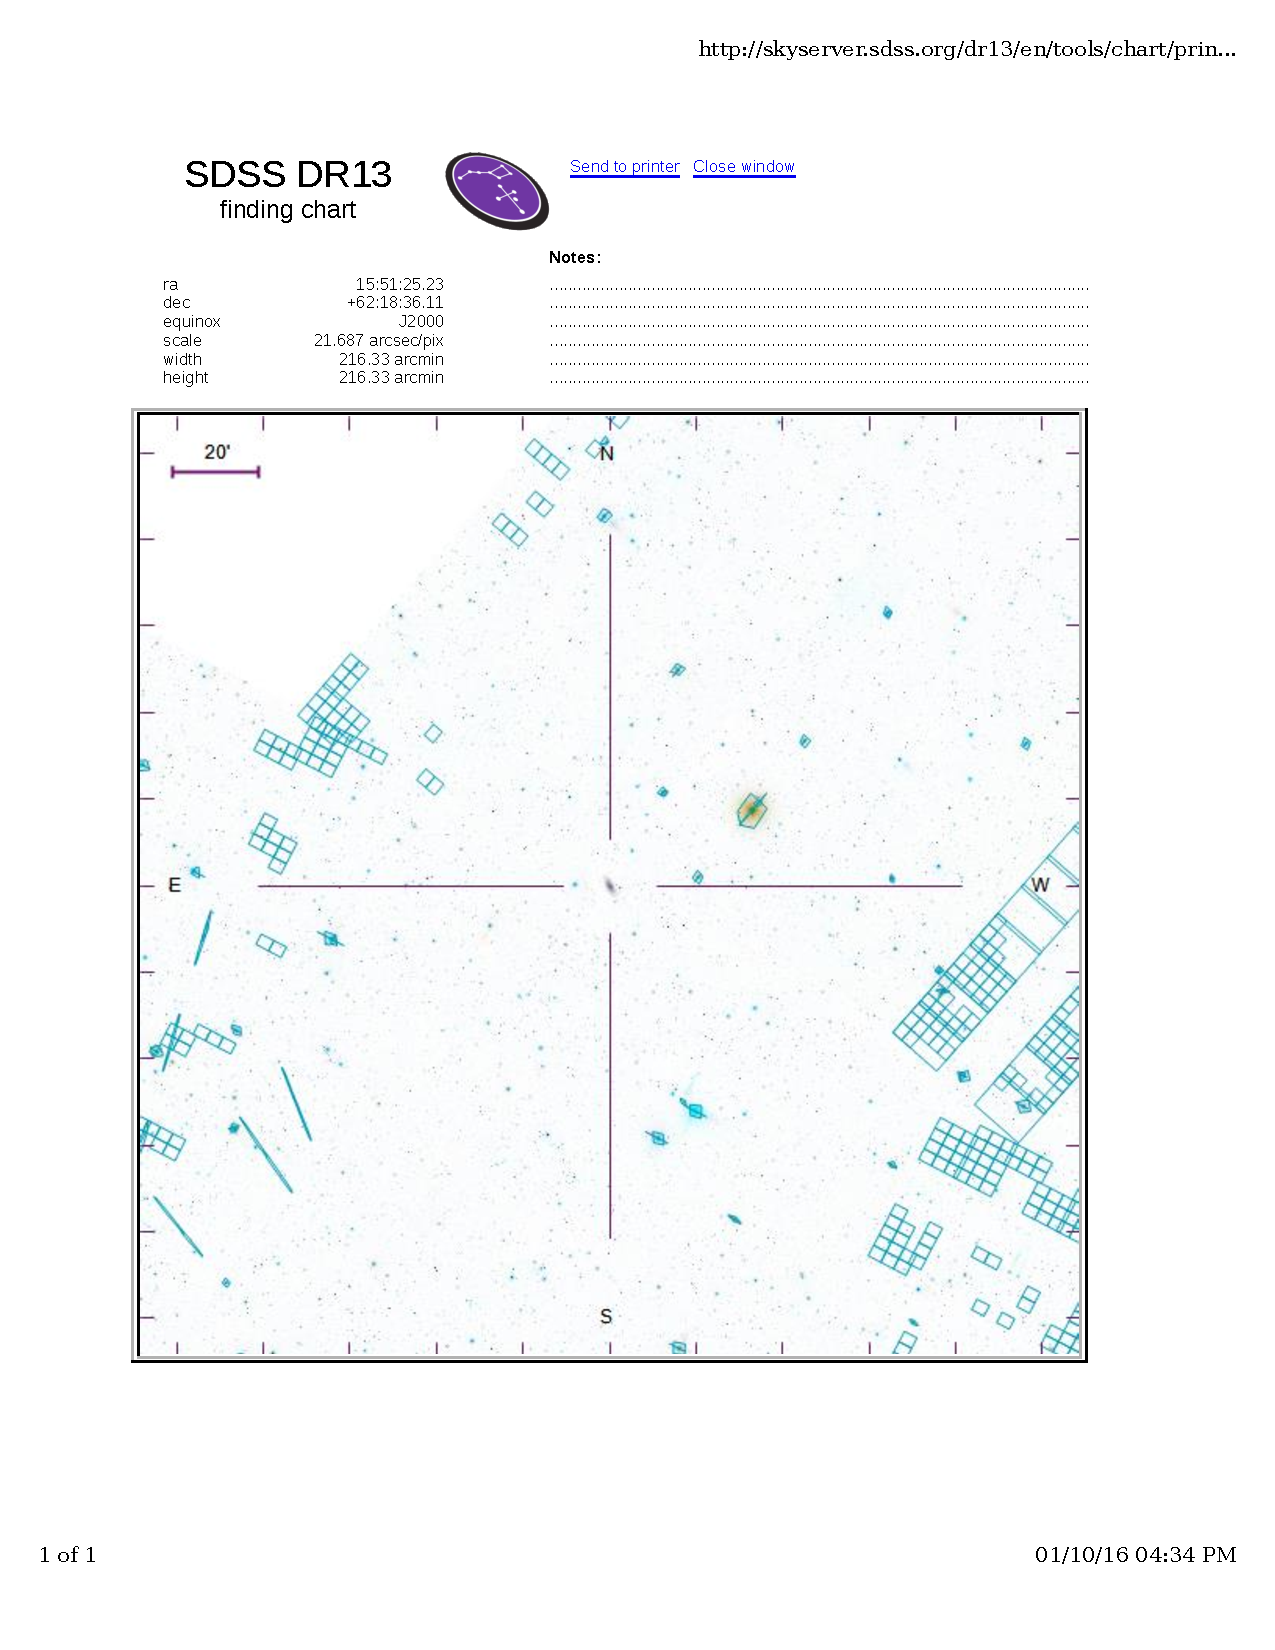
\includegraphics[scale=0.7]{figures/NGC6015.pdf}
\caption{NGC6015 SDSS DR8 Navigate Tool image with masks}
\end{figure}

\begin{figure}[h!]
\centering
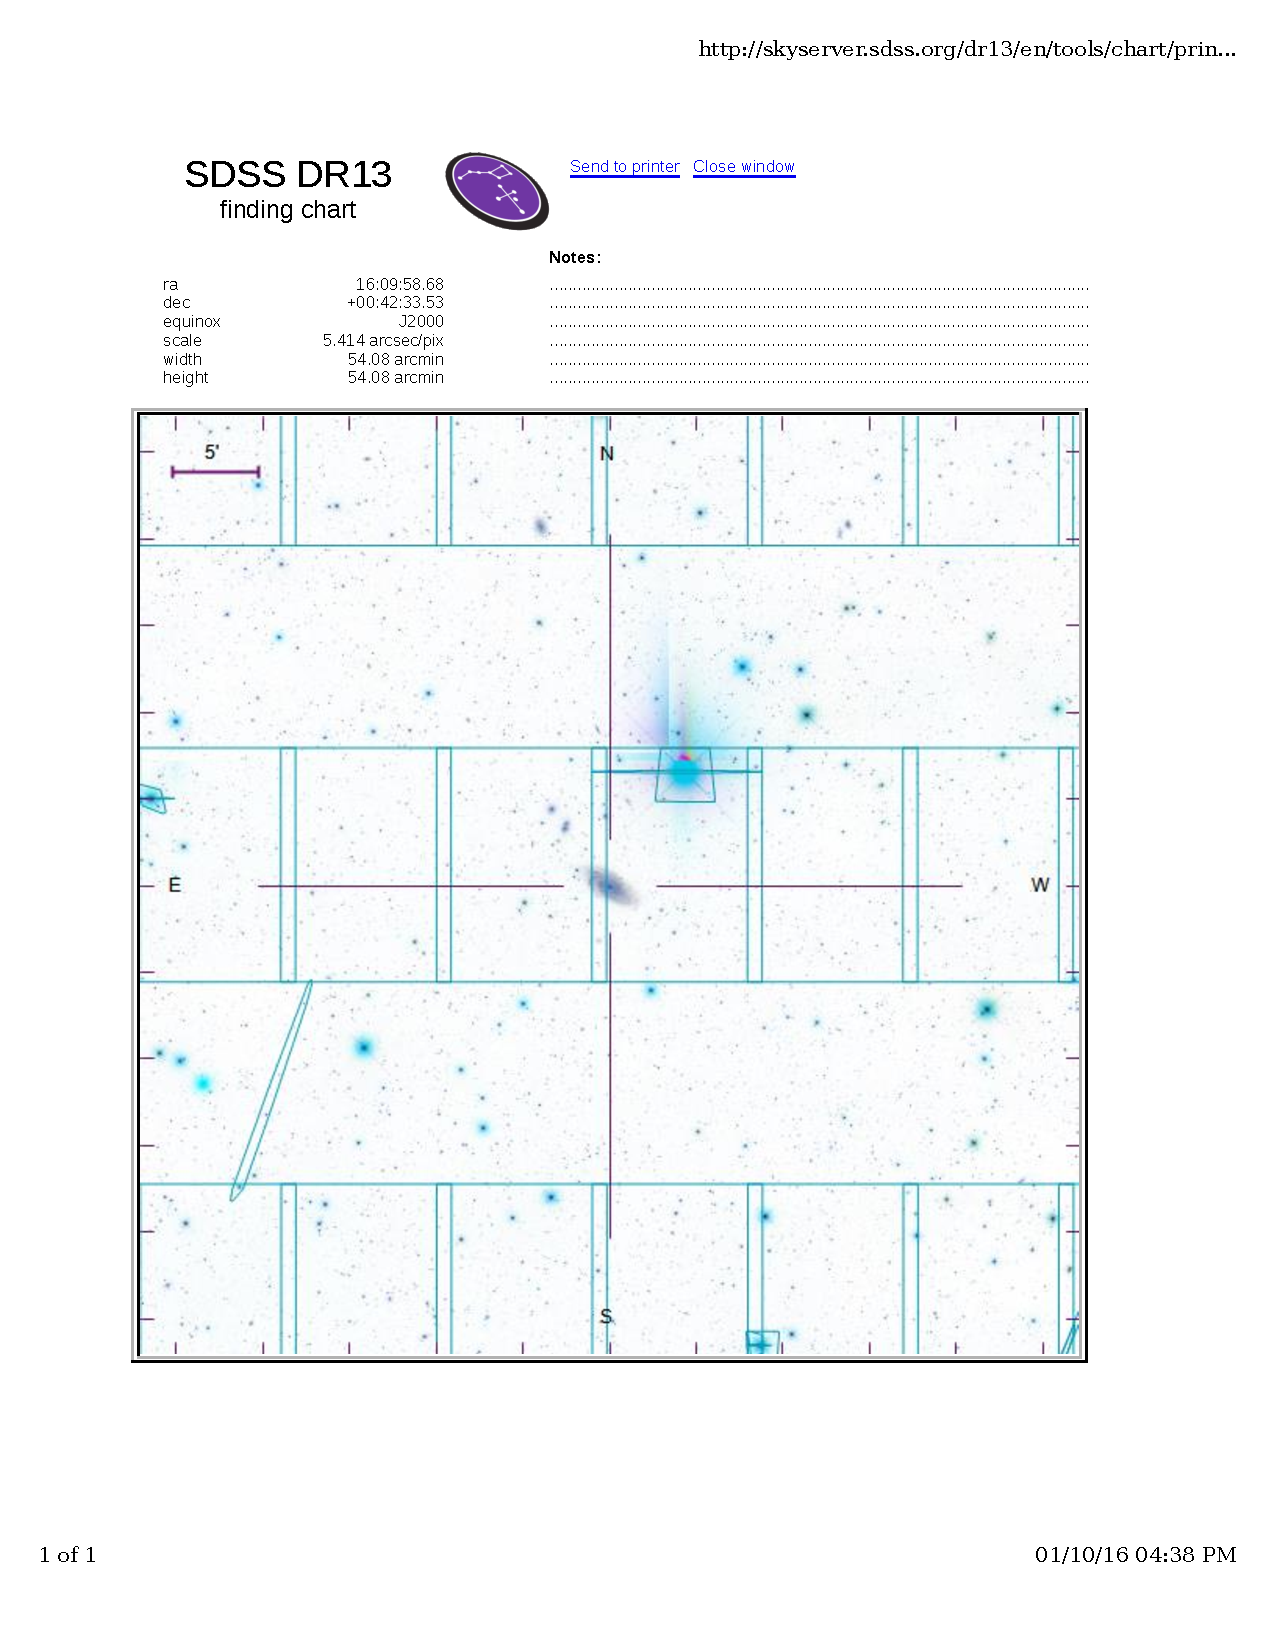
\includegraphics[scale=0.7]{figures/NGC6070.pdf}
\caption{NGC6070 SDSS DR8 Navigate Tool image with masks}
\end{figure}

\begin{figure}[h!]
\centering
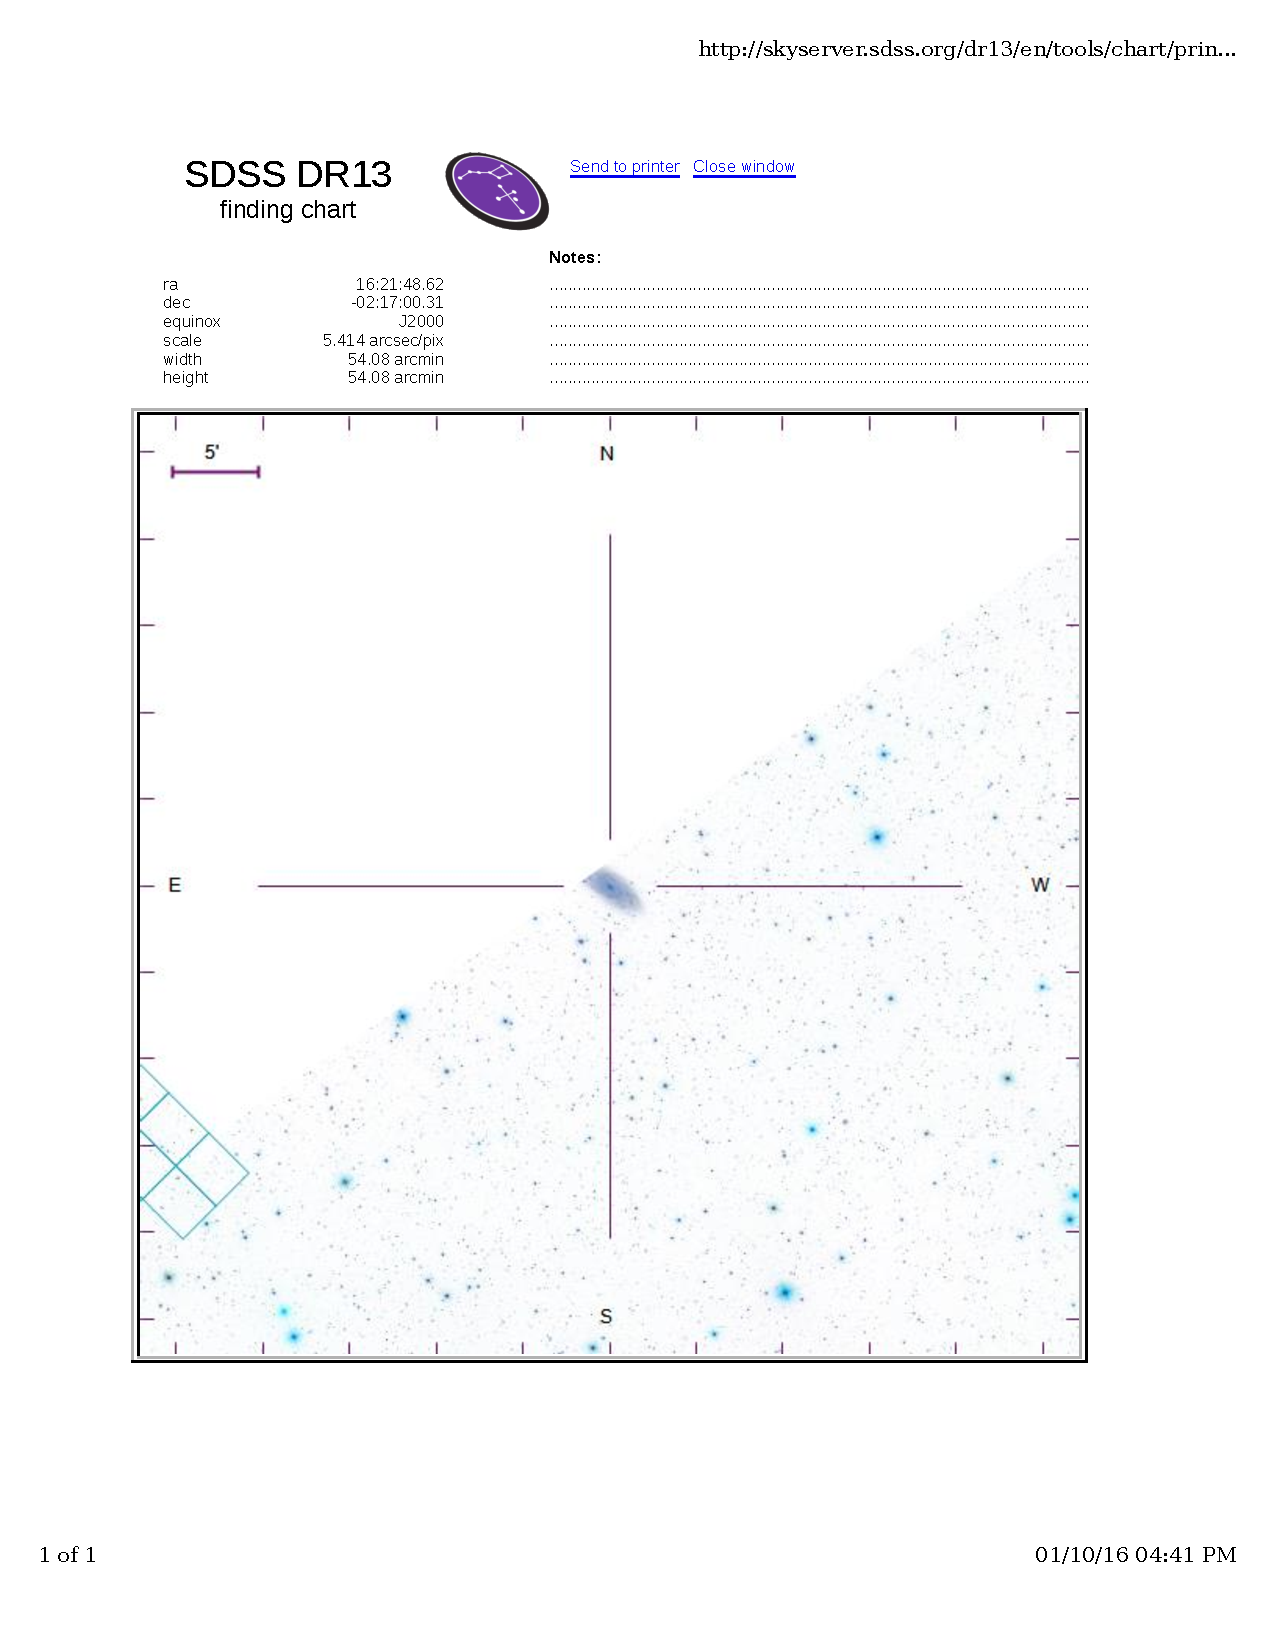
\includegraphics[scale=0.7]{figures/NGC6118.pdf}
\caption{NGC6118 SDSS DR8 Navigate Tool image with masks}
\end{figure}

\begin{figure}[h!]
\centering
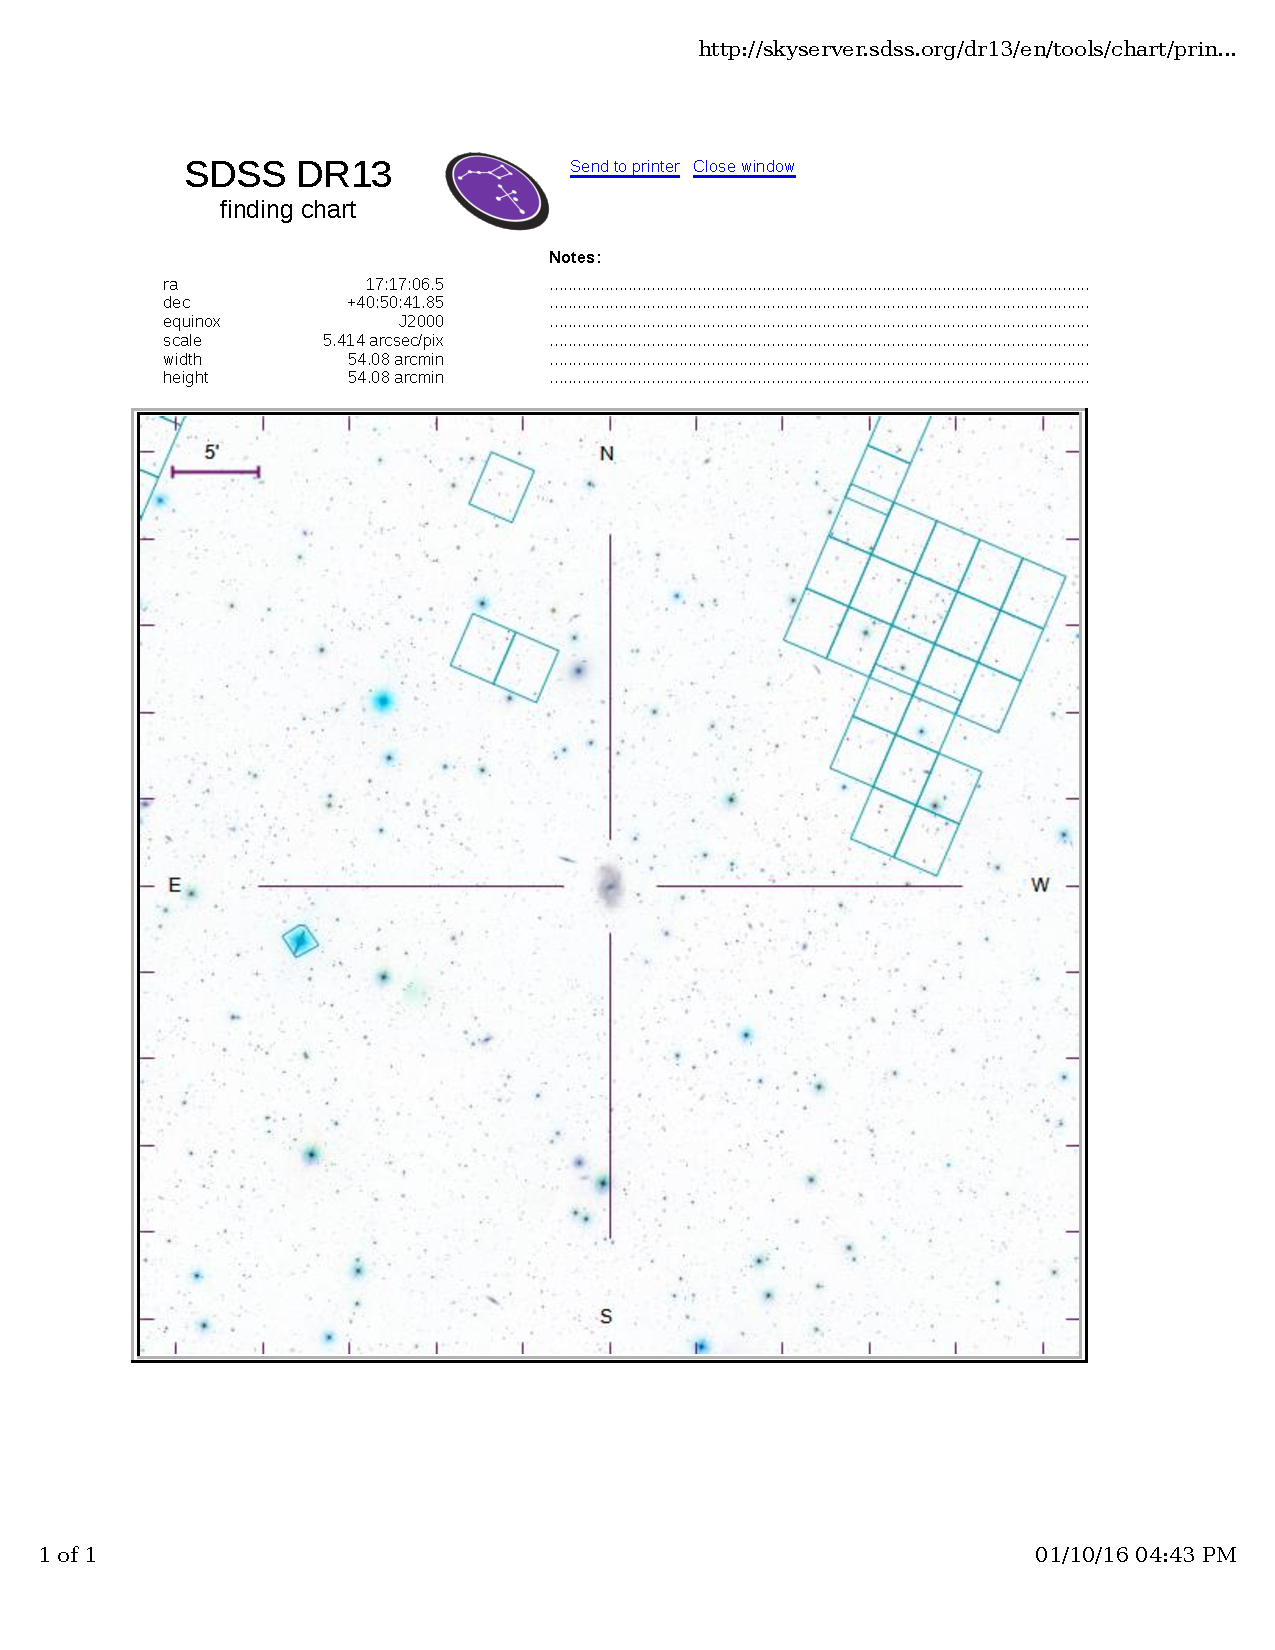
\includegraphics[scale=0.7]{figures/NGC6339.pdf}
\caption{NGC6339 SDSS DR8 Navigate Tool image with masks}
\end{figure}


\begin{figure}[h!]
\centering
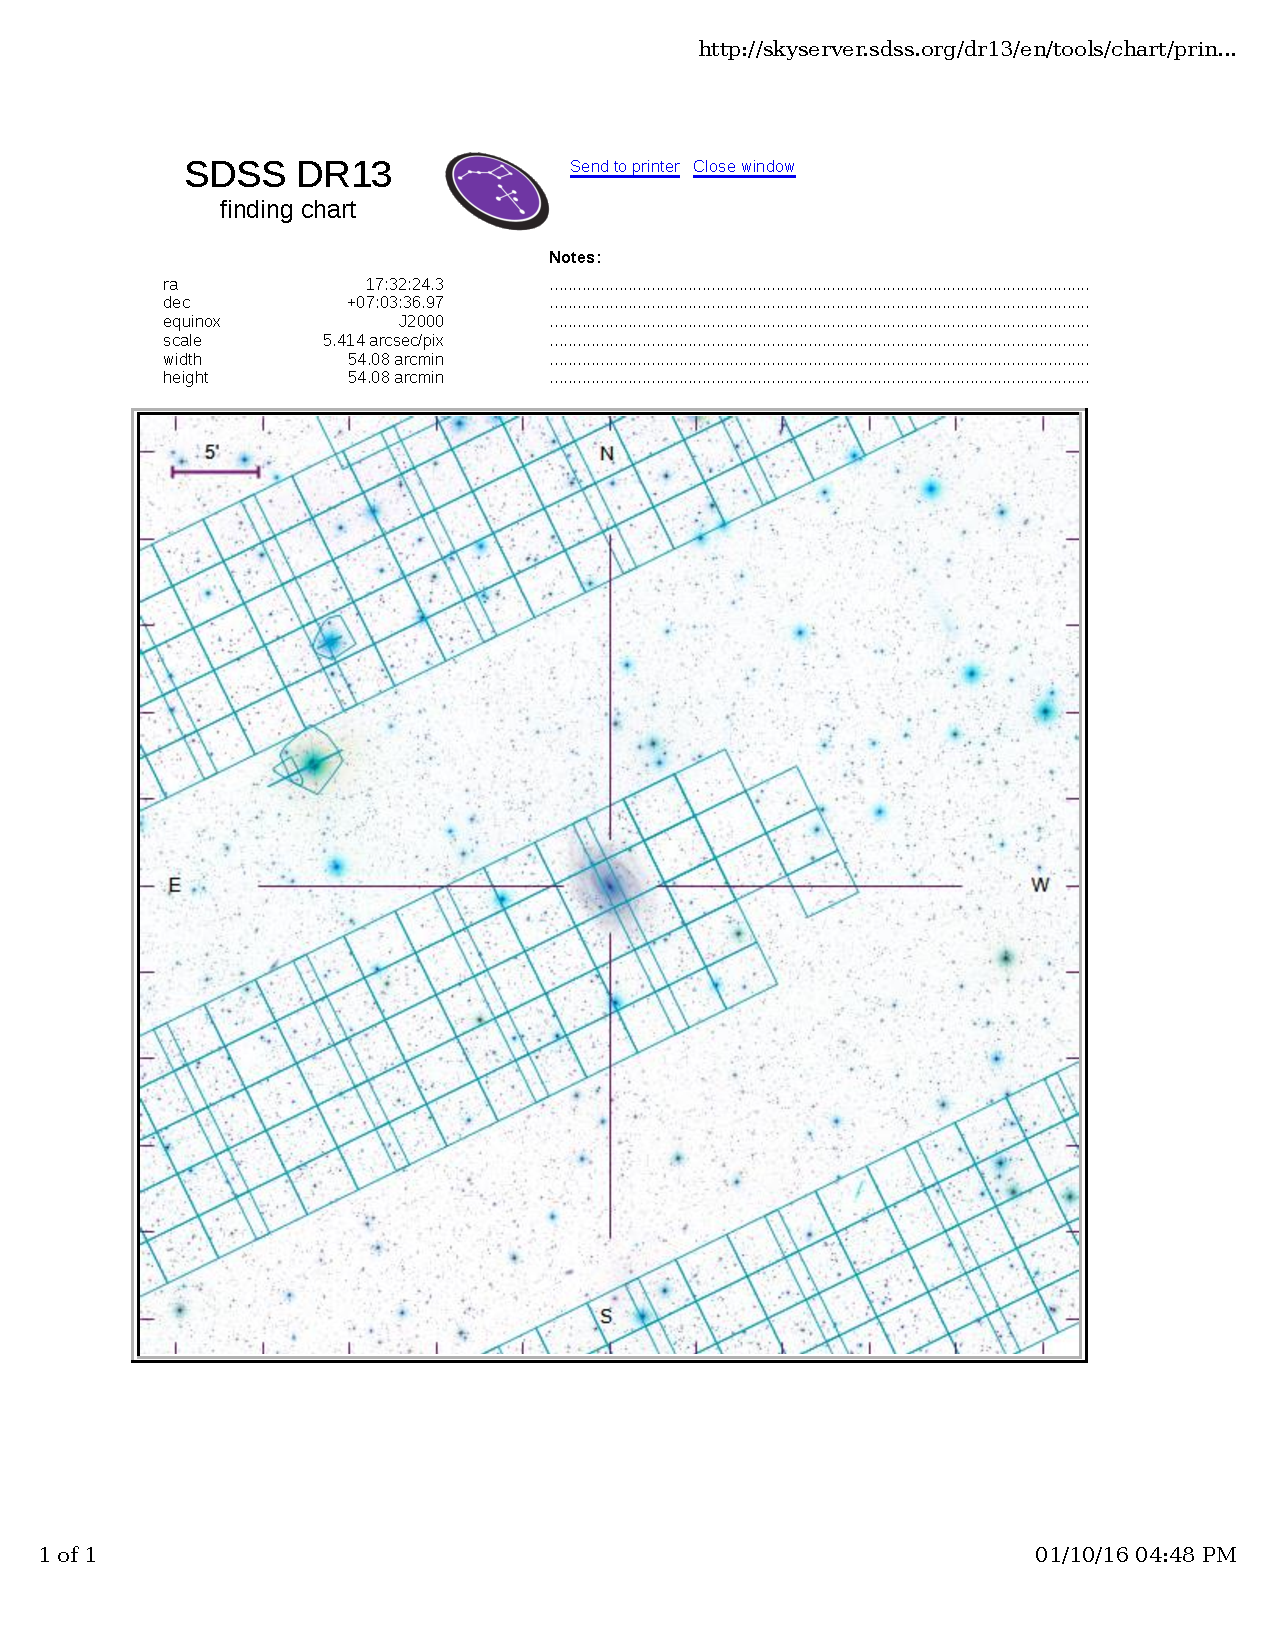
\includegraphics[scale=0.7]{figures/NGC6384.pdf}
\caption{NGC6384 SDSS DR8 Navigate Tool image with masks}
\end{figure}

\clearpage

\begin{figure}[h!]
\centering
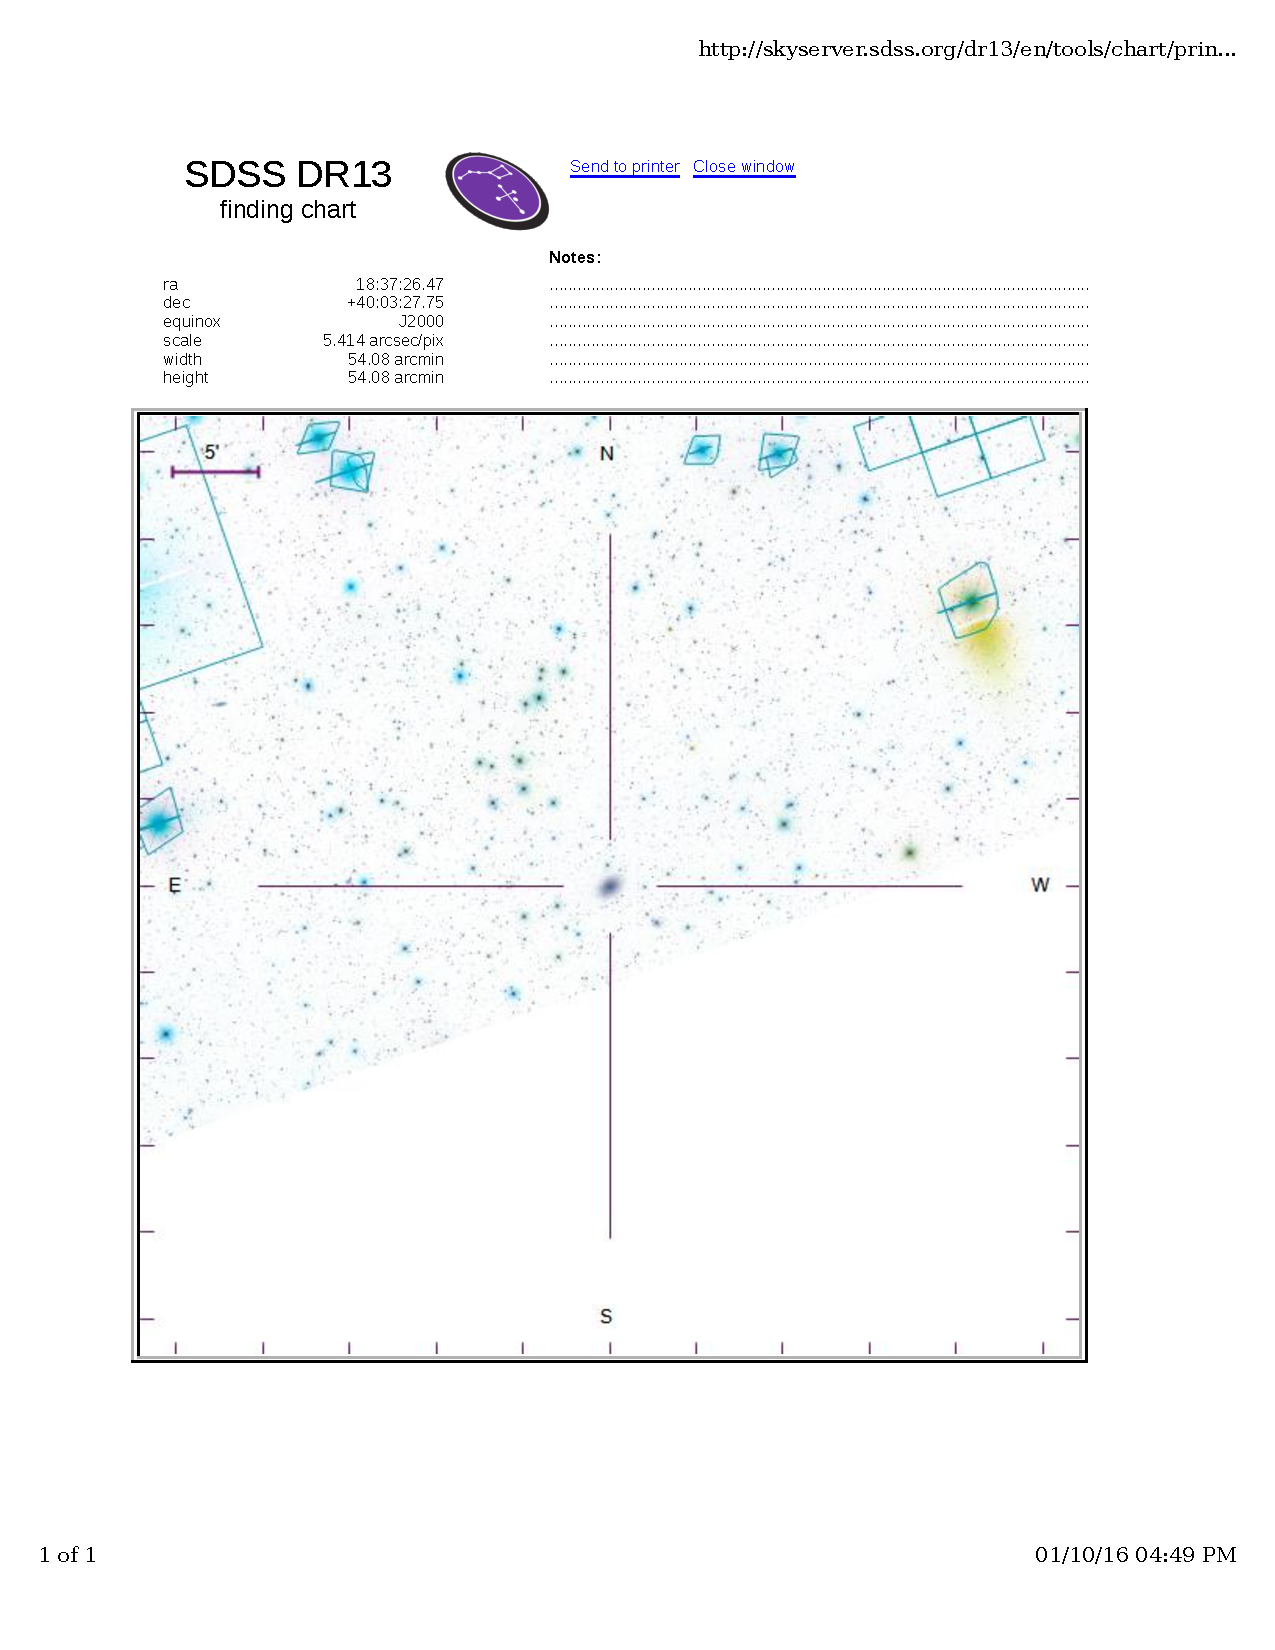
\includegraphics[scale=0.7]{figures/NGC6675.pdf}
\caption{NGC6675 SDSS DR8 Navigate Tool image with masks}
\end{figure}

\begin{figure}[h!]
\centering
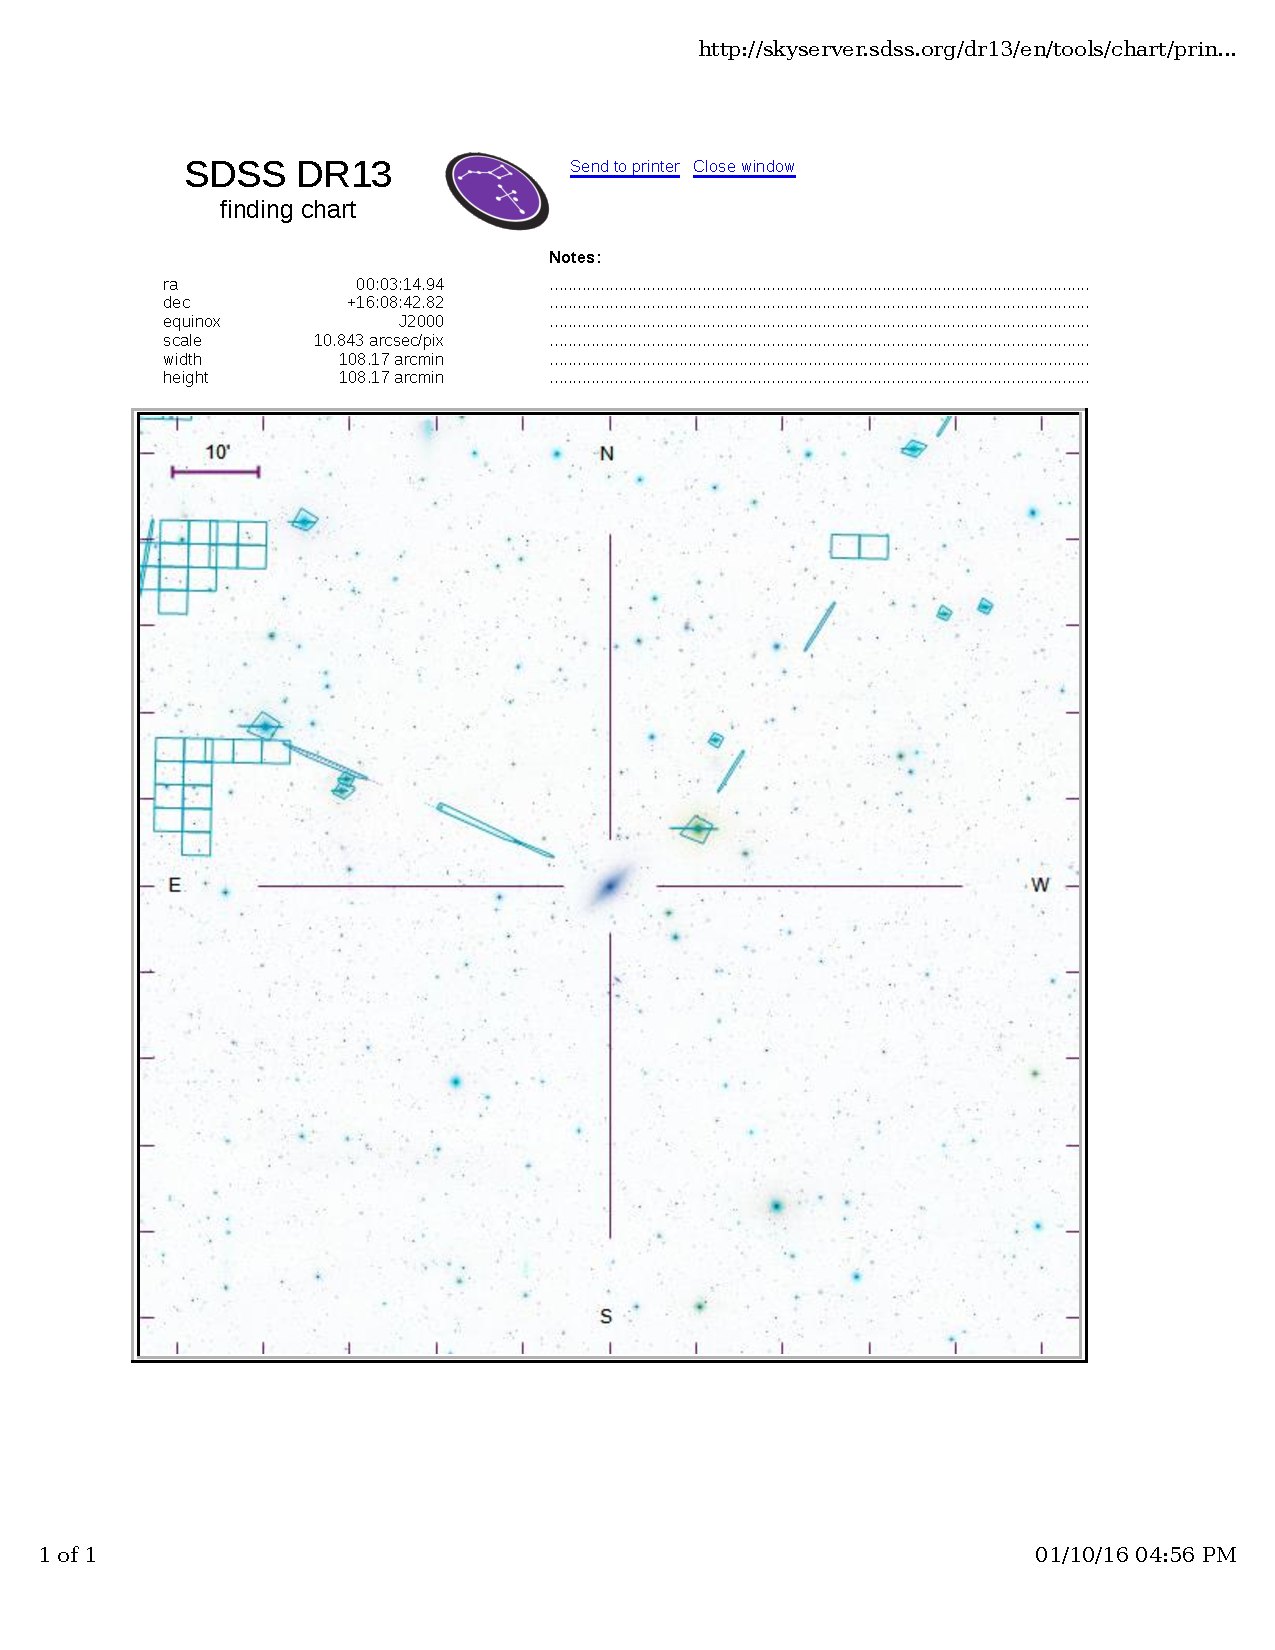
\includegraphics[scale=0.7]{figures/NGC7814.pdf}
\caption{NGC7814 SDSS DR8 Navigate Tool image with masks}
\end{figure}

\begin{figure}[h!]
\centering
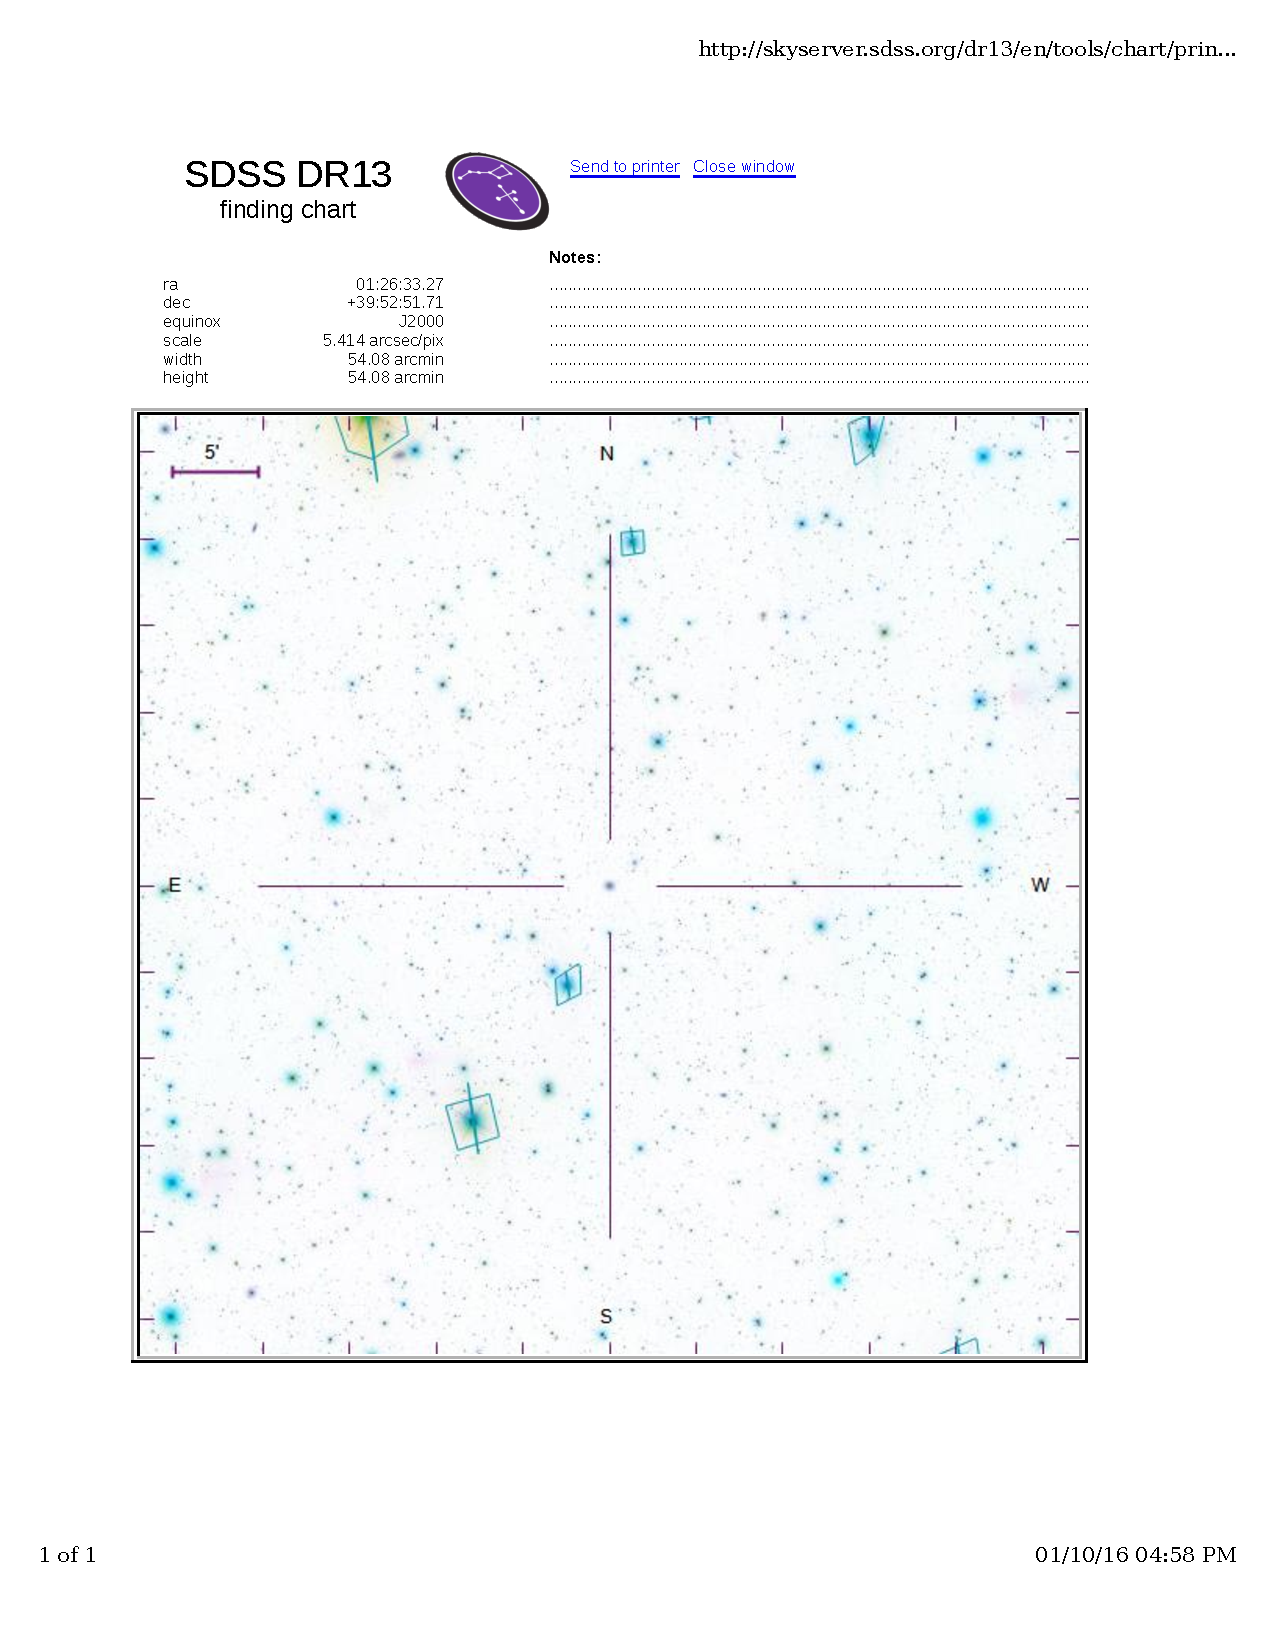
\includegraphics[scale=0.7]{figures/PGC005363.pdf}
\caption{PGC005363 SDSS DR8 Navigate Tool image with masks}
\end{figure}

\begin{figure}[h!]
\centering
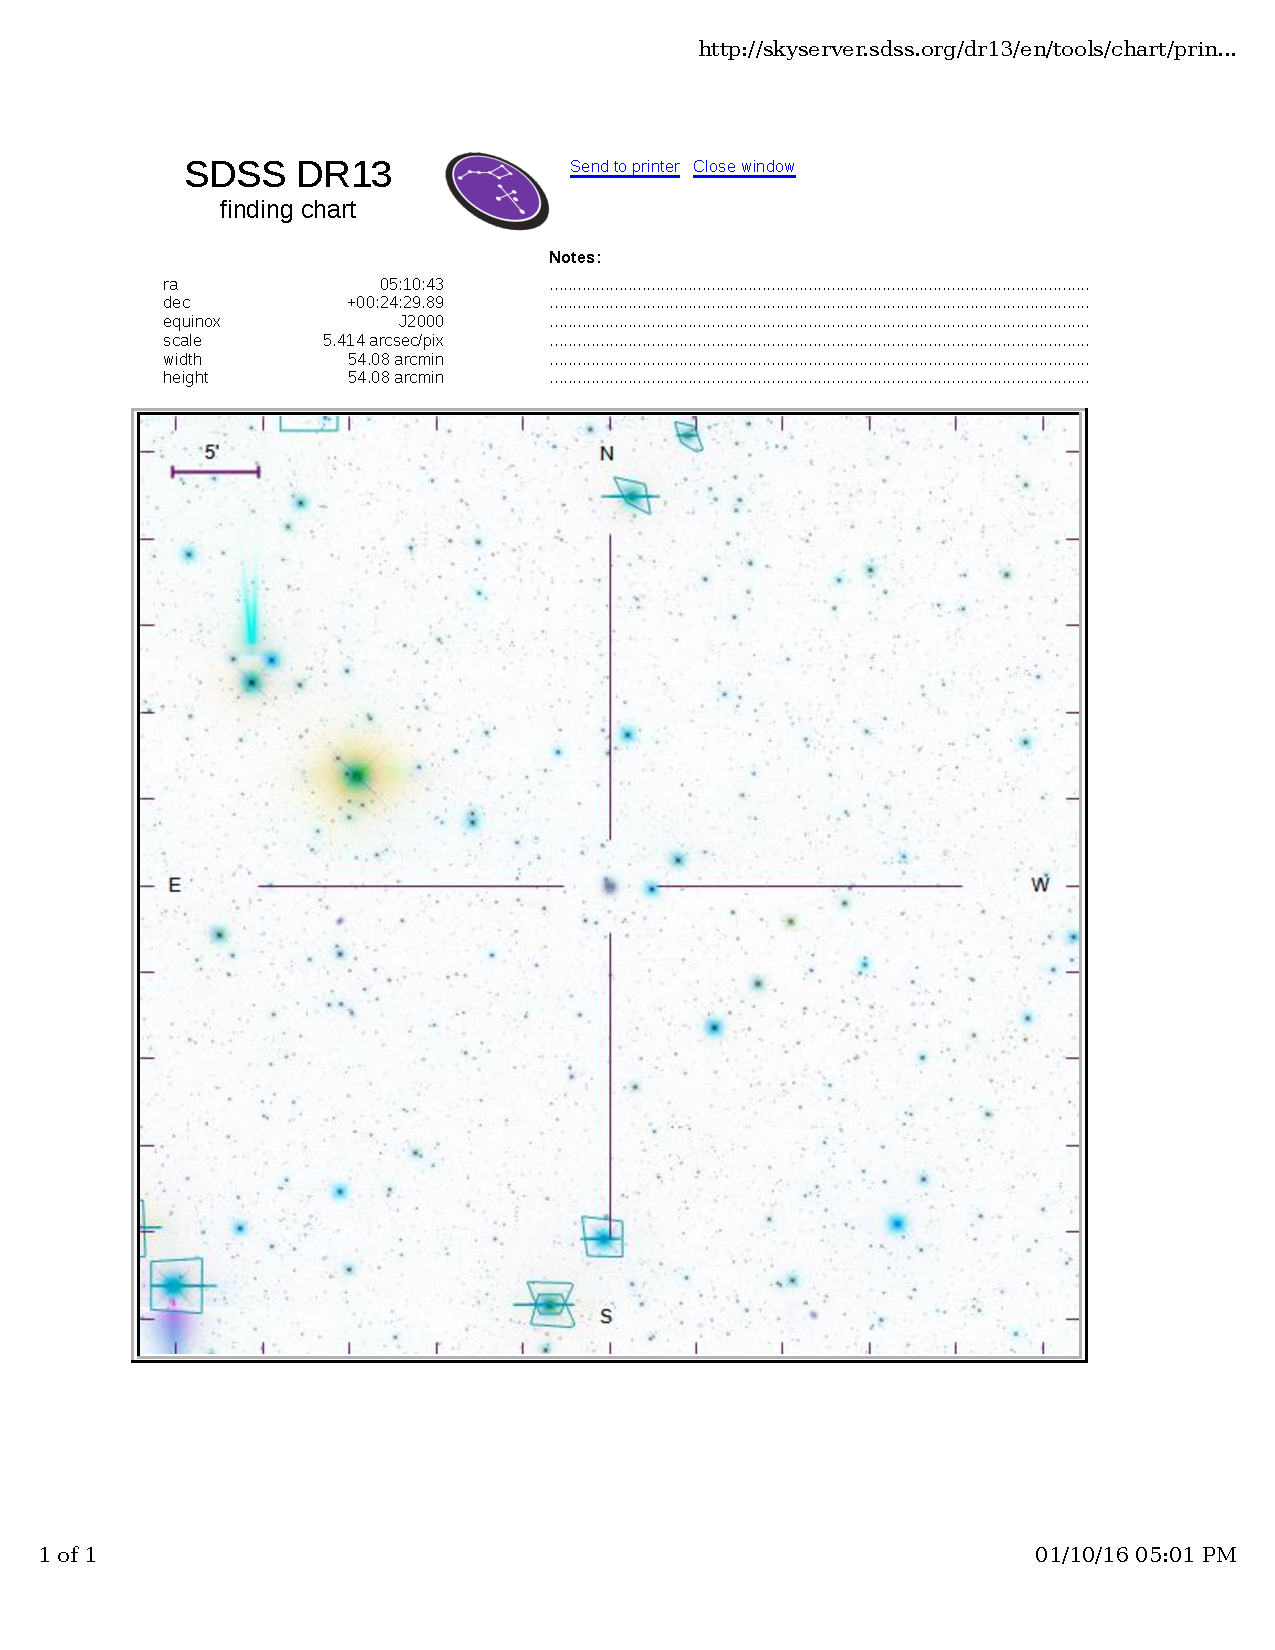
\includegraphics[scale=0.7]{figures/UGC03258.pdf}
\caption{UGC03258 SDSS DR8 Navigate Tool image with masks}
\end{figure}

\begin{figure}[h!]
\centering
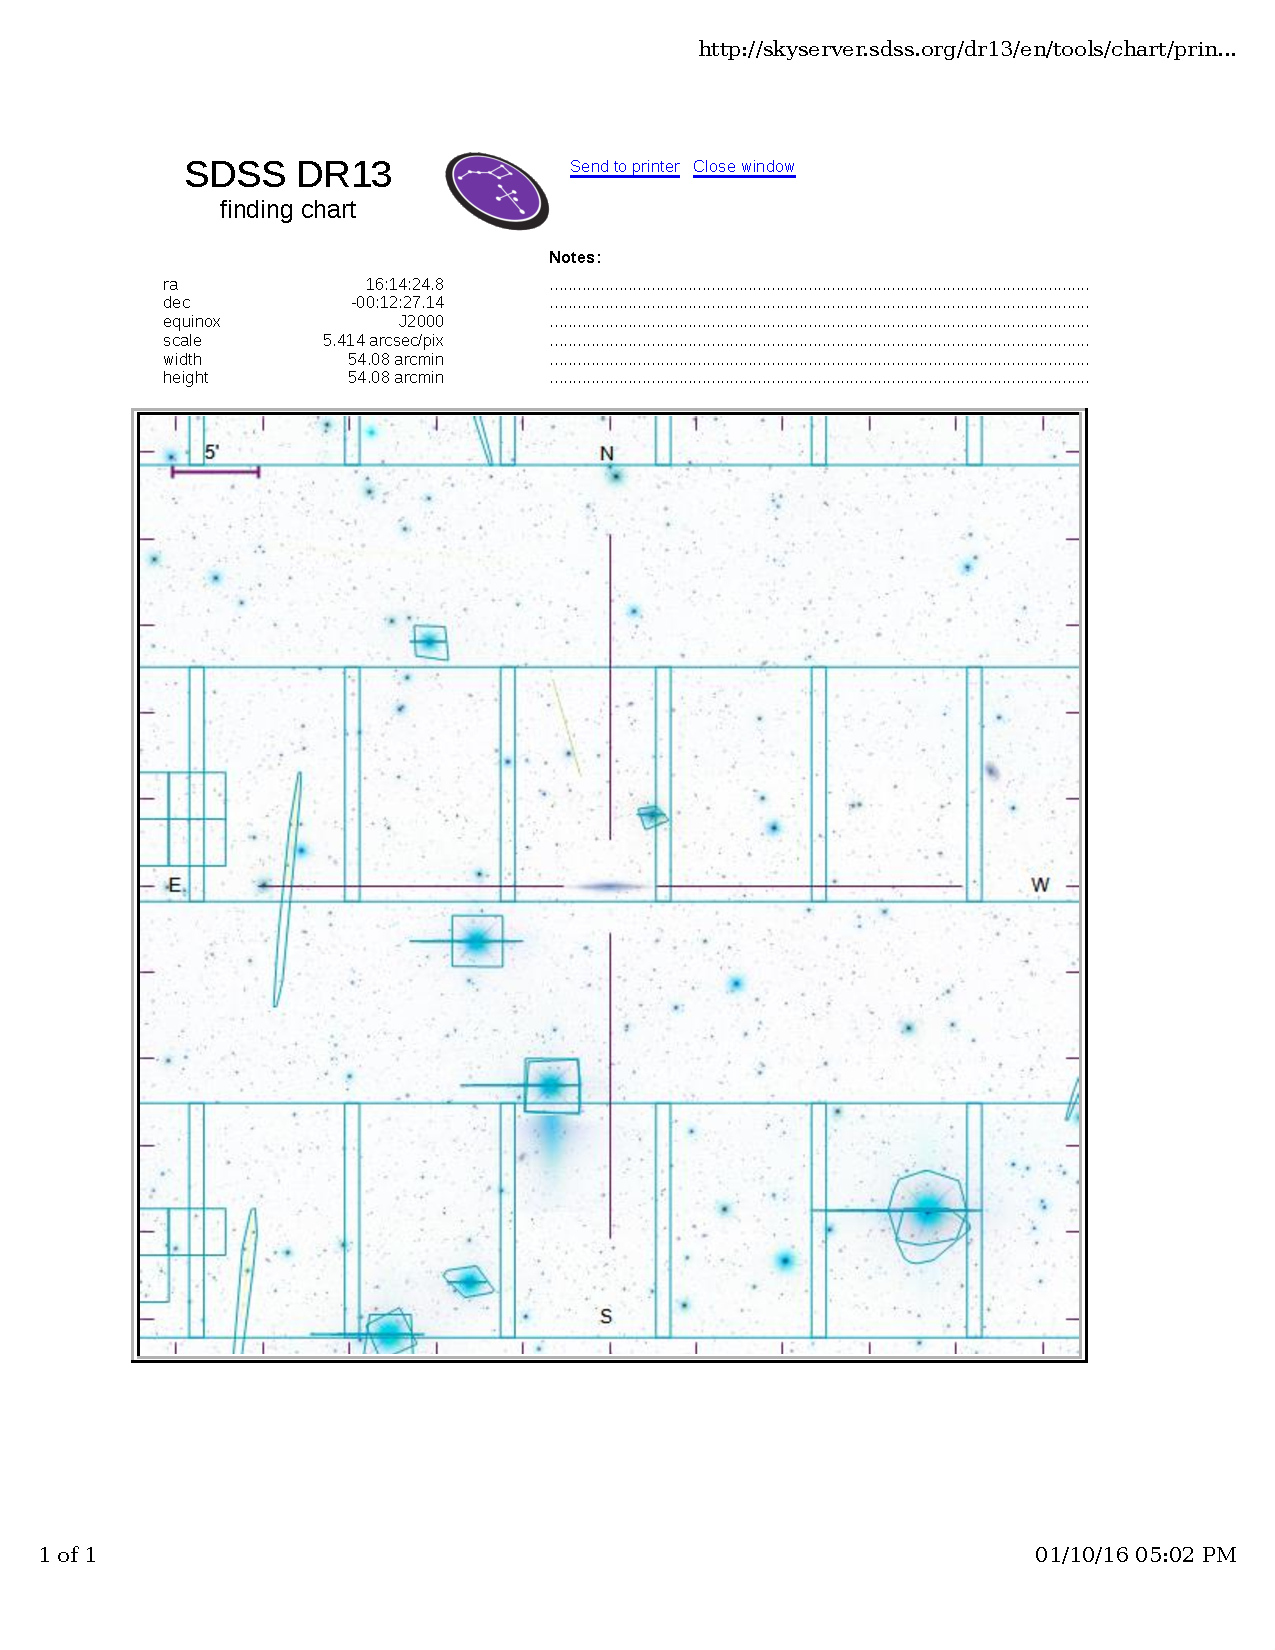
\includegraphics[scale=0.7]{figures/UGC10288.pdf}
\caption{UGC10288 SDSS DR8 Navigate Tool image with masks}
\end{figure}

\begin{figure}[h!]
\centering
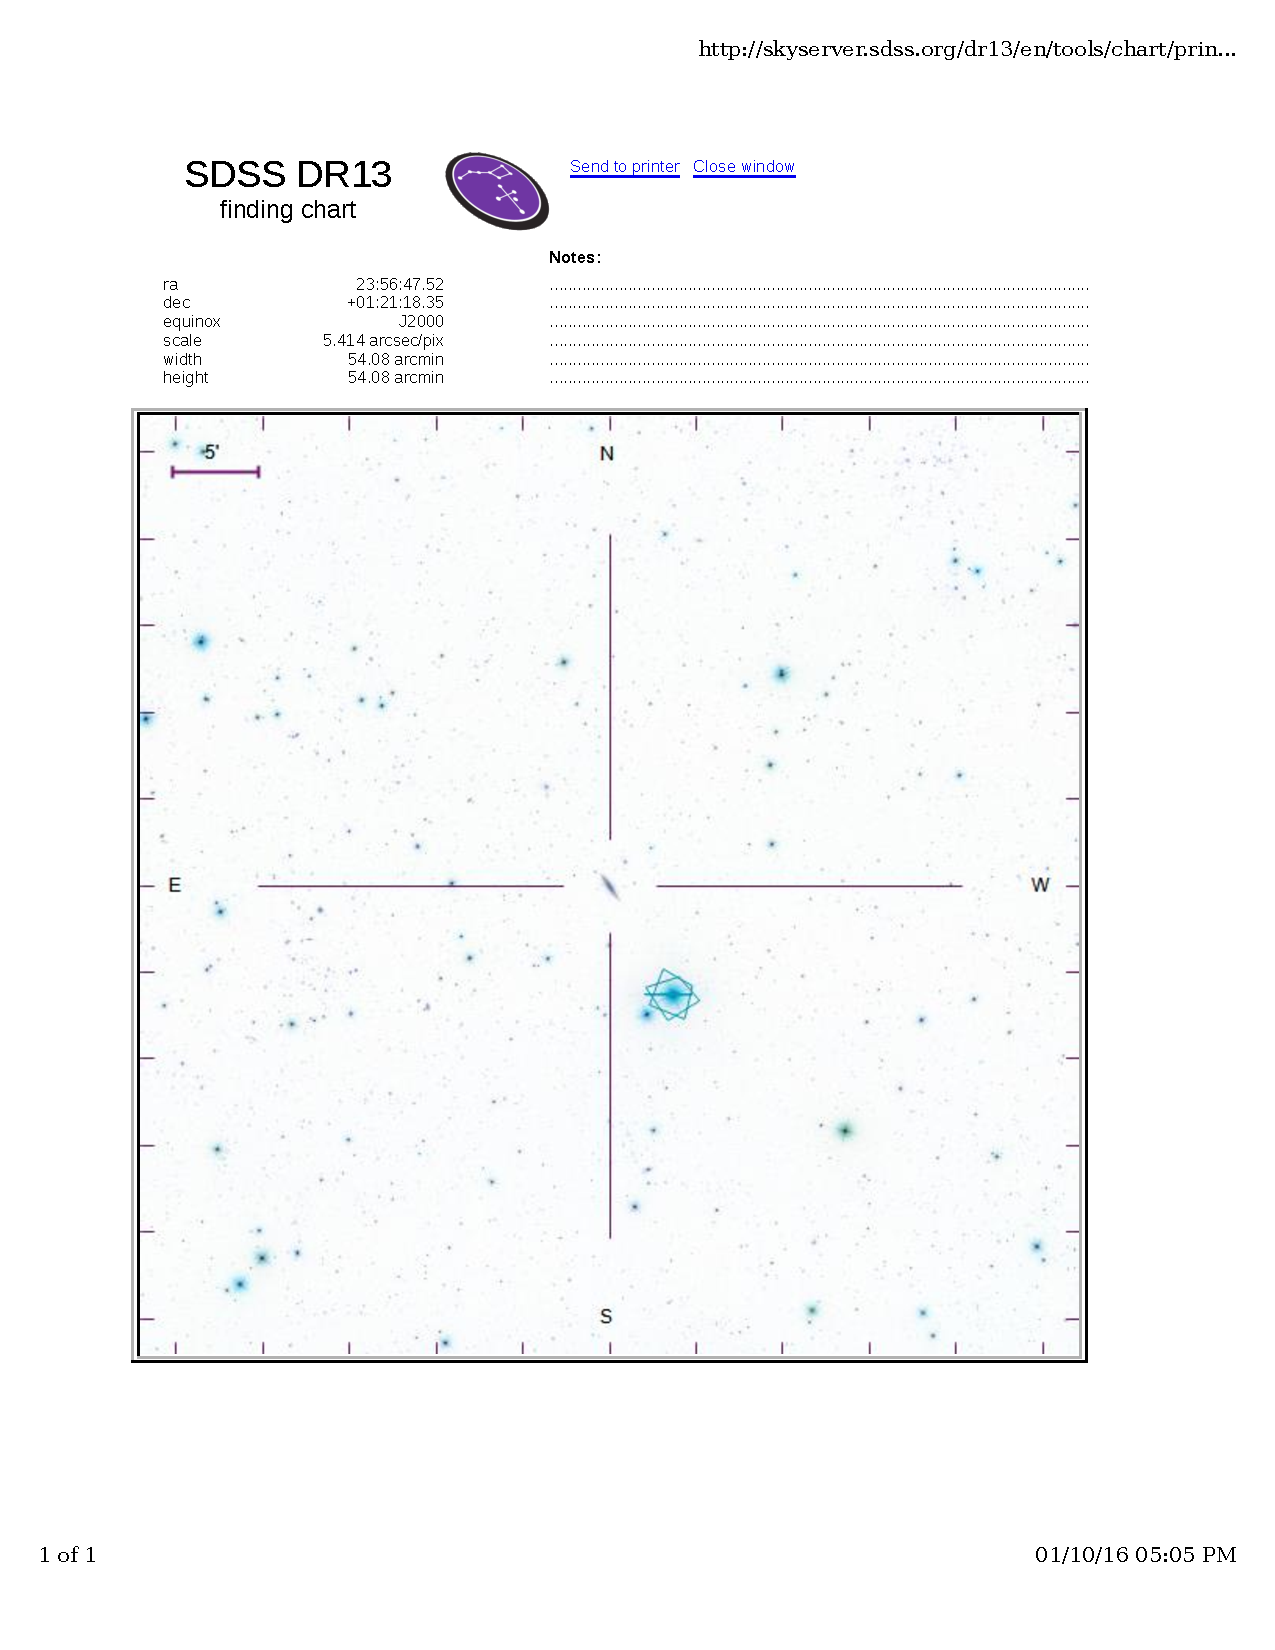
\includegraphics[scale=0.7]{figures/UGC12857.pdf}
\caption{UGC12857 SDSS DR8 Navigate Tool image with masks}
\end{figure}

\clearpage

\newpage
\center
\begin{thebibliography}{1}
\bibitem{image masks} Algorithms: Image masks. (n.d.). Retrieved October 02, 2016, from \url{https://www.sdss3.org/dr8/algorithms/masks.php}\\

\bibitem{Atlas3D} Cappellari, M., Emsellem, E., Krajnovi\'c, D., et al. 2011, MNRAS, 413, 813\\

\bibitem{classic SDSS} Classic Sloan Digital Sky Survey. (n.d.). Retrieved September 18, 2016, from \url{http://classic.sdss.org/}\\

\bibitem{dr9 masks} Creating a Large Scale Structure Galaxy Catalog. (n.d.). Retrieved October 02, 2016, from \url{https://www.sdss3.org/dr9/tutorials/lss_galaxy.php}\\

\bibitem{Vaucouleurs} de Vaucouleurs, G., de Vaucouleurs, A., Corwin, H. G., Jr., et al. 1991, Third
Reference Catalogue of Bright Galaxies (New York: Springer)\\

\bibitem{Fukugita} Fukugita, M., Shimasaku, K., \& Ichikawa, T. 1995, PASP, 107, 945\\

\bibitem{Great Circle Drift Scanning} Great Circle Drift Scanning. (n.d.). Retrieved September 25, 2016, from \url{http://classic.sdss.org/dr7/products/general/edr_html/node26.html}\\

\bibitem{mangle} Mangle: Overview. (n.d.). Retrieved October 02, 2016, from \url{http://space.mit.edu/~molly/mangle/}\\

\bibitem{NED 871} NED results for object(s) in publication ``2011MNRAS.413..813C" (n.d.). Retrieved September 21, 2016, from \url{https://ned.ipac.caltech.edu/cgi-bin/nph-objsearch?search_type=Search&refcode=2011MNRAS.413..813C}\\

\bibitem{NYUVAGC} NYU Value-Added Galaxy Catalog. (n.d.). Retrieved October 02, 2016, from \url{http://sdss.physics.nyu.edu/vagc/}\\

\bibitem{SDSS-III} SDSS-III. (n.d.). Retrieved September 20, 2016, from \url{https://www.sdss3.org/}\\

\bibitem{CrossID} SDSS CrossID for DR8. (n.d.). Retrieved September 26, 2016, from \url{http://cas.sdss.org/dr8/en/tools/crossid/crossid.asp}\\

\bibitem{navigate} SDSS DR8 Navigate Tool. (n.d.). Retrieved October 01, 2016, from \url{http://skyserver.sdss.org/dr8/en/tools/chart/navi.asp}\\

\bibitem{navigate DR13} SDSS DR13 Navigate Tool. (n.d.). Retrieved October 01, 2016, from \url{http://skyserver.sdss.org/dr13/en/tools/chart/navi.aspx}\\

\bibitem{scope} SDSS Scope. (n.d.). Retrieved September 20, 2016, from \url{http://www.sdss.org/dr13/scope/}\\

\bibitem{Survey Coordinates} SDSS Survey coordinates. (n.d.). Retrieved September 25, 2016, from \url{https://www.sdss3.org/dr10/algorithms/surveycoords.php}\\

\bibitem{SQL tutorial} Searching for Data: A Tutorial. (n.d.). Retrieved September 18, 2016, from \url{http://skyserver.sdss.org/dr12/en/help/howto/search/searchhowtohome.aspx}\\

\bibitem{2MASS} Skrutskie, M. F., Cutri, R. M., Stiening, R., et al. 2006, AJ, 131, 1163\\

\bibitem{DR7 sky coverage} Sky coverage. (n.d.). Retrieved September 25, 2016, from \url{http://classic.sdss.org/dr7/coverage/}\\

\bibitem{SDSS webpage} Sloan Digital Sky Surveys. (n.d.). Retrieved September 18, 2016, from \url{http://www.sdss.org/surveys/}\\

\bibitem{instruments} Telescopes and Instruments. (n.d.). Retrieved September 20, 2016, from \url{http://www.sdss.org/instruments/}\\

\bibitem{DR8} The Eighth SDSS Data Release (DR8). (n.d.). Retrieved September 20, 2016, from \url{https://www.sdss3.org/dr8/}\\

\bibitem{DR9} The Ninth SDSS Data Release (DR9). (n.d.). Retrieved September 20, 2016, from \url{https://www.sdss3.org/dr9/}\\

\bibitem{SDSS} York, D. G., Adelman, J., Anderson, J. E., Jr., et al. 2000, AJ, 120, 1579\\

\bibitem{schema} Schema Browser. (n.d.). Retrieved September 18, 2016, from \url{http://skyserver.sdss.org/dr12/en/help/browser/browser.aspx}\\

\end{thebibliography}

\end{document}